%% LaTeX2e class for student theses
%% sections/evaluation.tex
%% 
%% Karlsruhe Institute of Technology
%% Institute for Program Structures and Data Organization
%% Chair for Software Design and Quality (SDQ)
%%
%% Dr.-Ing. Erik Burger
%% burger@kit.edu
%%
%% Version 1.3.3, 2018-04-17

\chapter{Modellierung}
\label{ch:modellierung}
Wie bereits in \autoref{sec:eventbasetransformation} beschrieben, bietet das PCM die Möglichkeit, eventbasierte Kommunikation zu modellieren und auch eine konkrete MOM-Architektur zu modellieren, die mithilfe einer Modelltransformation in die Systemarchitektur eingewoben wird. Diese Modellierung hat das Problem, dass die Kommunikation nur in eine Richtung funktioniert, wie in \autoref{img:oldEventBased}a zu sehen ist. Ein Sender sendet eine Nachricht an einen Empfänger. Auf dem Weg dorthin durchläuft die Nachricht eine Komponentenkette und wird mit bestimmten Ressourcenanforderungen belegt. Der Empfänger erhält schließlich die Nachricht. Da in diesem Szenario eine explizit modellierte Warteschlange fehlt, ist es nicht möglich bestimmte Effekte abzudecken, zum Beispiel den Füllstand der Warteschlange und die damit eingehende Auswirkung auf die Latenz einer Nachricht. In \autoref{img:oldEventBased}b ist eine Warteschlange explizit modelliert um damit solche Effekte abdecken zu können. Dabei sendet der Sender die Nachricht an die MOM, diese sortiert die Nachricht in die entsprechende Warteschlange ein und ein Empfänger holt die Nachricht ab, sobald er die Ressourcen dazu hat. Dieses Szenario ist mit der aktuellen eventbasierten Kommunikation in PCM nicht darstellbar, weil kein Abholen einer Nachricht vorgesehen ist. Deshalb soll im Folgenden eine Modellierung präsentiert werden, die eine explizite Warteschlange und ein Verteilsystem, das Nachrichten an passenden Warteschlangen verteilt, modelliert.\par
Dazu wird zunächst mithilfe einer Anforderungserhebung in \autoref{sec:anforderungserhebung} Anforderungen gesammelt werden, die eine solche Modellierung erfüllen soll. Im Anschluss wird in \autoref{sec:modell} die Modellierung einer MOM vorgestellt, die die Anforderungen erfüllen soll. In \autoref{sec:rmqRd} soll das Modell mithilfe der in \autoref{sec:rmqBenchmark} ausgemessenen MOM kalibriert werden. Ziel dabei ist, dass das kalibrierte Modell sich wie die echte MOM verhält und die Einflussfaktoren, die dabei identifiziert wurden, auch sichtbar werden. Dazu wird in \autoref{sec:performanceanalyse} das MOM-Modell in mehreren Simulationen eingesetzt und mit den realem Messungen verglichen. 
\begin{figure}
\center
  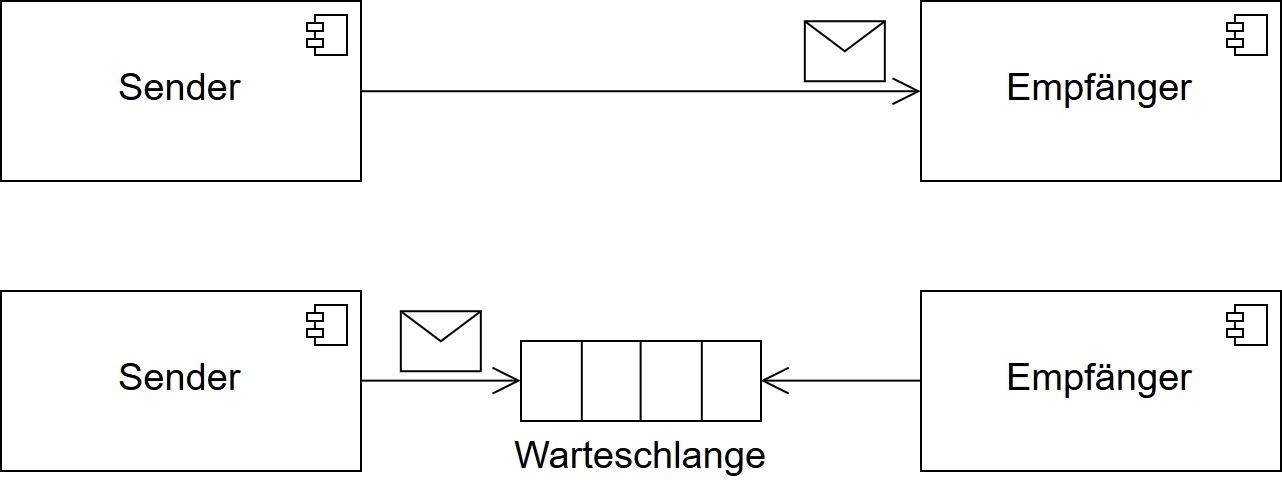
\includegraphics[width=1\textwidth]{images/modelling/oldEventBased.png}
  \caption{Aktuelle und gewünschte eventbasierte-Kommunikation}
  \label{img:oldEventBased}
\end{figure}


\section{Anforderungserhebung}
\label{sec:anforderungserhebung}
Basierend auf der Spezifizierung von MOMs aus \autoref{ch:Grundlagen} und den Messungen aus \autoref{ch:mom} wurden die folgenden Anforderungen an eine Modellierung abgeleitet. Dabei wurde zwischen technischen Anforderungen und Anforderungen an die Nutzbarkeit unterschieden. 
Zu den technischen Anforderungen gehören:
\begin{itemize}
    %\item Die Modellierung soll das allgemeine Verhalten einer MOM abbilden können.
    \item Asynchrones Senden und Empfangen von Nachrichten.
    \item Nachrichten können an eine bestimmte Warteschlange oder Topic gesendet werden.
    \item Das Modell sollte sich dafür eignen, verschiedene Nachrichtenraten abgebilden zu können
    \item Der Füllstand der Warteschlange soll mithilfe der Performance-Analyse ermittelt werden können.
    \item Die Latenz einer Nachricht soll mithilfe der Performance-Analyse ermittelt werden können.
\end{itemize}
Der Benutzer der Modellierung muss in der Lage sein, die folgenden Dinge angeben zu können:
\begin{itemize}
    \item Die Nachrichtengröße
    \item Die Topic einer Nachricht
\end{itemize}

%Angabe des Durchsatzes \\


%Das Ziel ist es eine allgemeine MOM Modellierung zu erstellen, die das Verhalten einer MOM abbilden kann. Dabei soll nicht Wert auf ein spezielles Verhalten gelegt werden. Stattdessen soll es moeglich sein die Modellierung um Konfigurationen, wie zum Beispiel RMQs lazy Queues, erweitern zu koennen. 

\section{Modell}
\label{sec:modell}
Im Folgenden soll eine Modellierung einer MOM präsentiert werden, die die zuvor definierten Anforderungen erfüllt. Dabei war nicht das Ziel eine Meta-Modell Erweiterung zu erstellen, sondern mit bereits existierenden PCM-Elementen zu arbeiten. Diese wurden in \autoref{ch:Grundlagen} beschrieben. Dazu wird zu jeder PCM-Rolle beschrieben, wie die Modellierung aussieht.

%Anhand der bekannten MOM Architekturen aus der Untersuchung verschiedener MOMs wurde versucht zu definieren wie eine MOM modelliert werden kann. Dabei wurden die Anforderungen versucht umzusetzen. \\
%- 2 Moeglichkeiten entweder mit oder ohne Exchange explizit zu modellieren.\\
%- Vorteil Explizit: RDs fuer verteilung (konnte aber nicht ausgemessen werden) \\
%- Nachrichten Typen mitschicken (fanout, direct) und in Branches auswerten

\subsection{Repository}
Das Repository wird vom Komponentenentwickler verwendet um neue Komponenten zu erstellen und vom Systemarchitekt um Komponenten zu entnehmen. Die untersuchte MOM Architektur besteht aus einem Verteiler und einer Warteschlange. Deshalb wurden die in \autoref{img:mom_repository} abgebildeten Komponenten und Schnittstellen definiert. Die Schnittstelle nach außen ist die \emph{IExchange} Schnittstelle. Diese bietet zwei Signaturen an. Eine zum Empfangen (\emph{receive}) und eine zum Senden (\emph{distribute}) einer Nachricht. Beide Methoden werden von der Komponente \emph{Exchange} angeboten. \emph{IQueue} ist die zweite Schnittstelle. Diese bietet auch zwei Signaturen an. Eine um eine Nachricht in eine Warteschlange abzulegen (\emph{put}) und eine weitere die eine Nachricht aus der Warteschlange entnimmt (\emph{get}). Diese Schnittstelle wird von der Komponente \emph{Queue} angeboten. Diese Komponenten, die eine Warteschlange abbilden soll, besitzt eine \emph{PassiveResource} die das Verhalten einer Warteschlange simulieren soll. Eine Passive Ressouce wird verwendet um das akquirieren und freigeben von Speicher zu simulieren. Dabei wird das Ablegen in die Warteschlange als \emph{release}-Aktion auf die passive Ressource und das entnehmen aus der Warteschlange als \emph{aquire}-Aktion auf die passive Ressource modelliert. Die \emph{Exchange}-Komponente benötigt eine Komponente die die \emph{IQueue}-Schnittstelle anbietet. Die Idee ist, dass alle Warteschlangen die benötigt werden von der \emph{Exchange}-Komponente benötigt werden. In \autoref{img:mom_repository} sind das aktuell zwei Warteschlangen. Mithilfe des RDSEFFs kann die \emph{Exchange}-Komponente zwischen den Warteschlangen wechseln. Dies ist in \autoref{img:queueBranch} dargestellt. Dabei wird mithilfe eines \emph{GuardedBranch} geprüft an welche Warteschlange die ankommenden Nachricht gehen soll. Der Fall, dass eine Nachricht aus der Warteschlange entnommen wird funktioniert genauso. Der Einsatz eines \emph{GuardedBranch} hat den Vorteil, dass das Modell weniger Modellelemente besitzt, anstatt dass jeder Sender und Empfänger mit jeder Warteschlange verbunden wäre.


%Dieser Ansatz ermöglicht es jedoch nicht einzelne Nachrichten durch das System zu verfolgen. \\


\begin{figure}
\center
  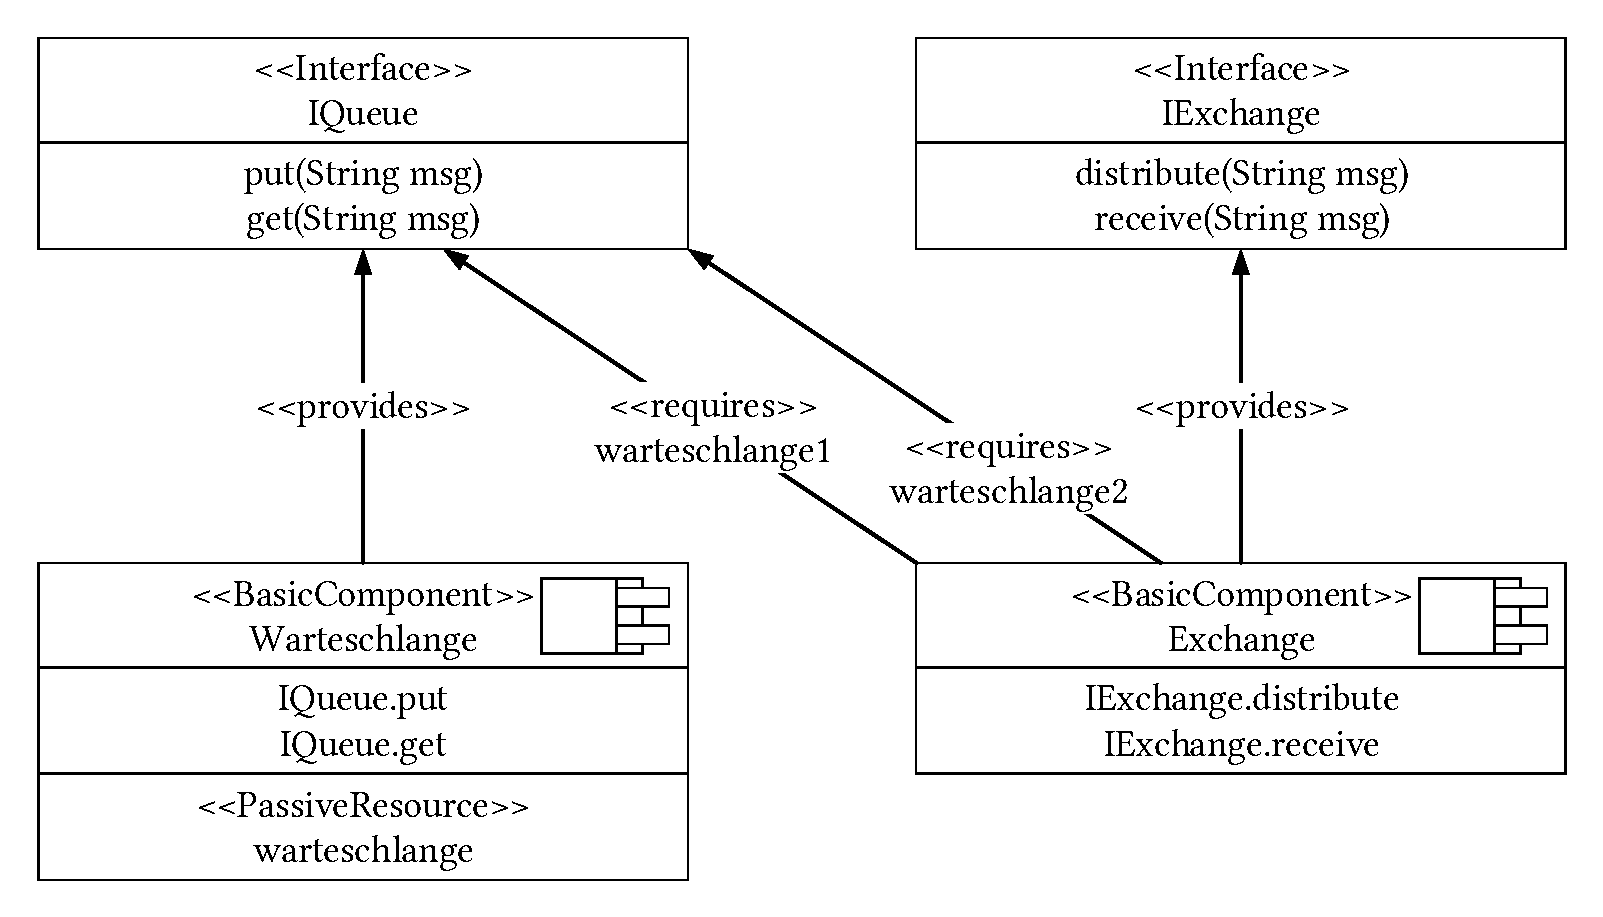
\includegraphics[width=1\textwidth]{images/modelling/modelingRepository.pdf}
  \caption{Repository-Modell einer MOM mit Exchange und Warteschlange}
  \label{img:mom_repository}
\end{figure}

\begin{figure}
\center
  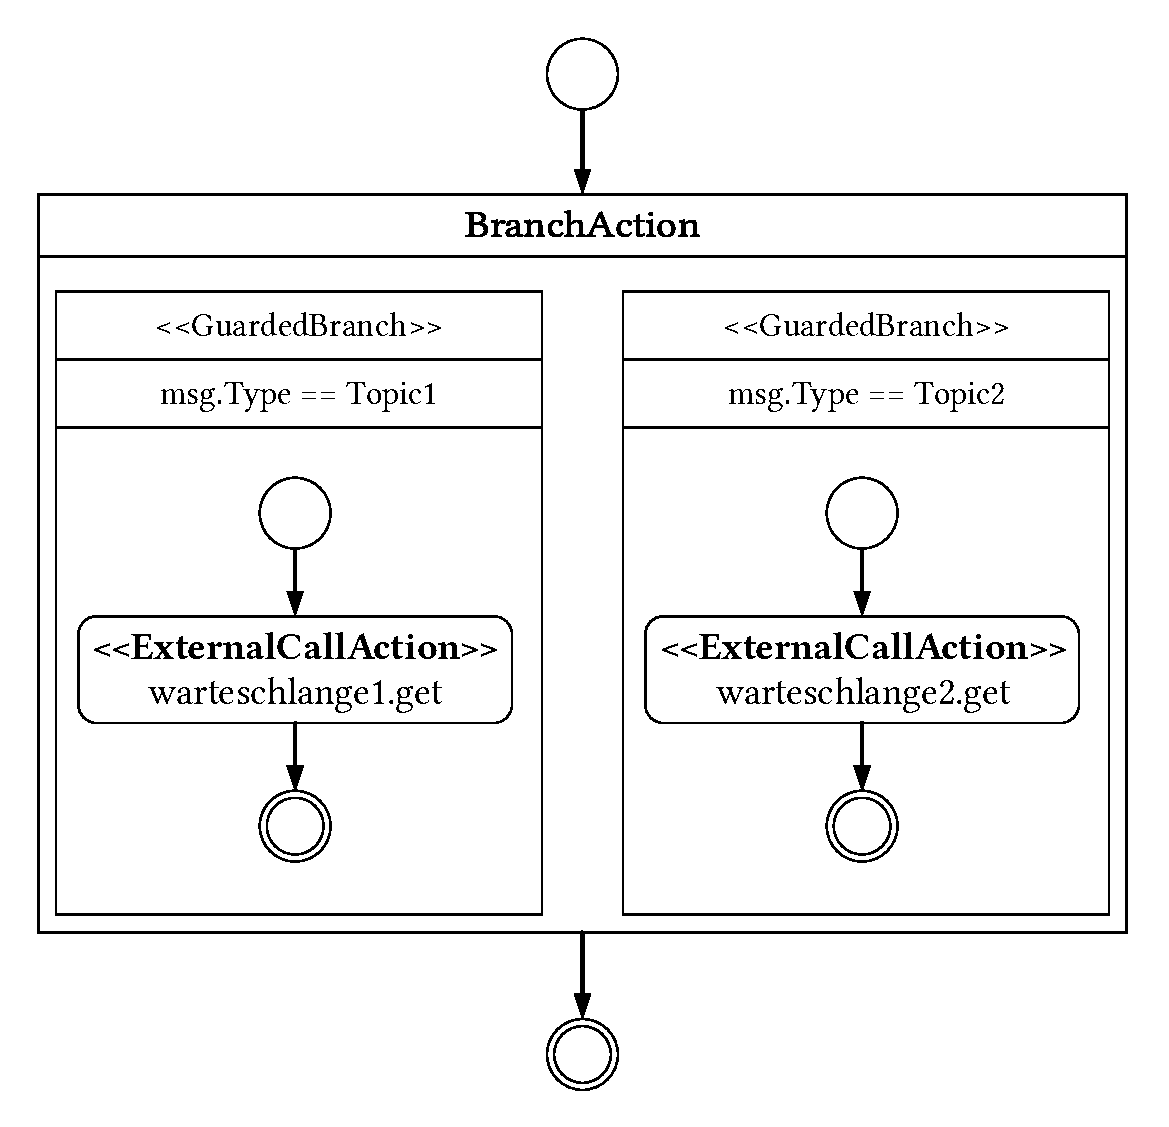
\includegraphics[width=0.7\textwidth]{images/modelling/modelingGuardedBranch.pdf}
  \caption{\emph{GuardedBranch} des \texttt{Exchange.receive} SEFF}
  \label{img:queueBranch}
\end{figure}

\subsection{System}
Im Systemmodell werden die einzelnen Komponenten aus dem Repository-Modell vom Softwarearchitekten zu einem System zusammengesetzt. Der Software-Architekt kann nun die Komponenten aus dem zuvor definierten Repository-Modell zusammensetzen. Dabei kann er zunächst entscheiden, wie viele Exchange-Komponenten im System existieren sollen. Wie auch in RMQ kann eine MOM aus mehreren Exchanges bestehen, die sich auf unterschiedlichen Maschinen befinden können. An einen Exchange werden dann die dazugehörigen Warteschlangen angeschlossen. Da ein Exchange eine Schnittstelle zum Senden und Empfangen von Nachrichten anbietet, können beliebig viele Sender- und Empfänger-Komponenten an einen Exchange angeschlossen werden. In \autoref{img:mom_system} ist ein Systemmodell mit zwei Exchange-Komponenten abgebildet. Dabei hat \emph{Exchange1} zwei Warteschlangenkomponenten und \emph{Exchange2} nur eine Warteschlange angeschlossen. Außerdem sind an \emph{Exchange1} je ein Sender und Empfänger angeschlossen. An \emph{Exchange2} sind zwei Sender und ein Empfänger angeschlossen. 

\begin{figure}
\center
  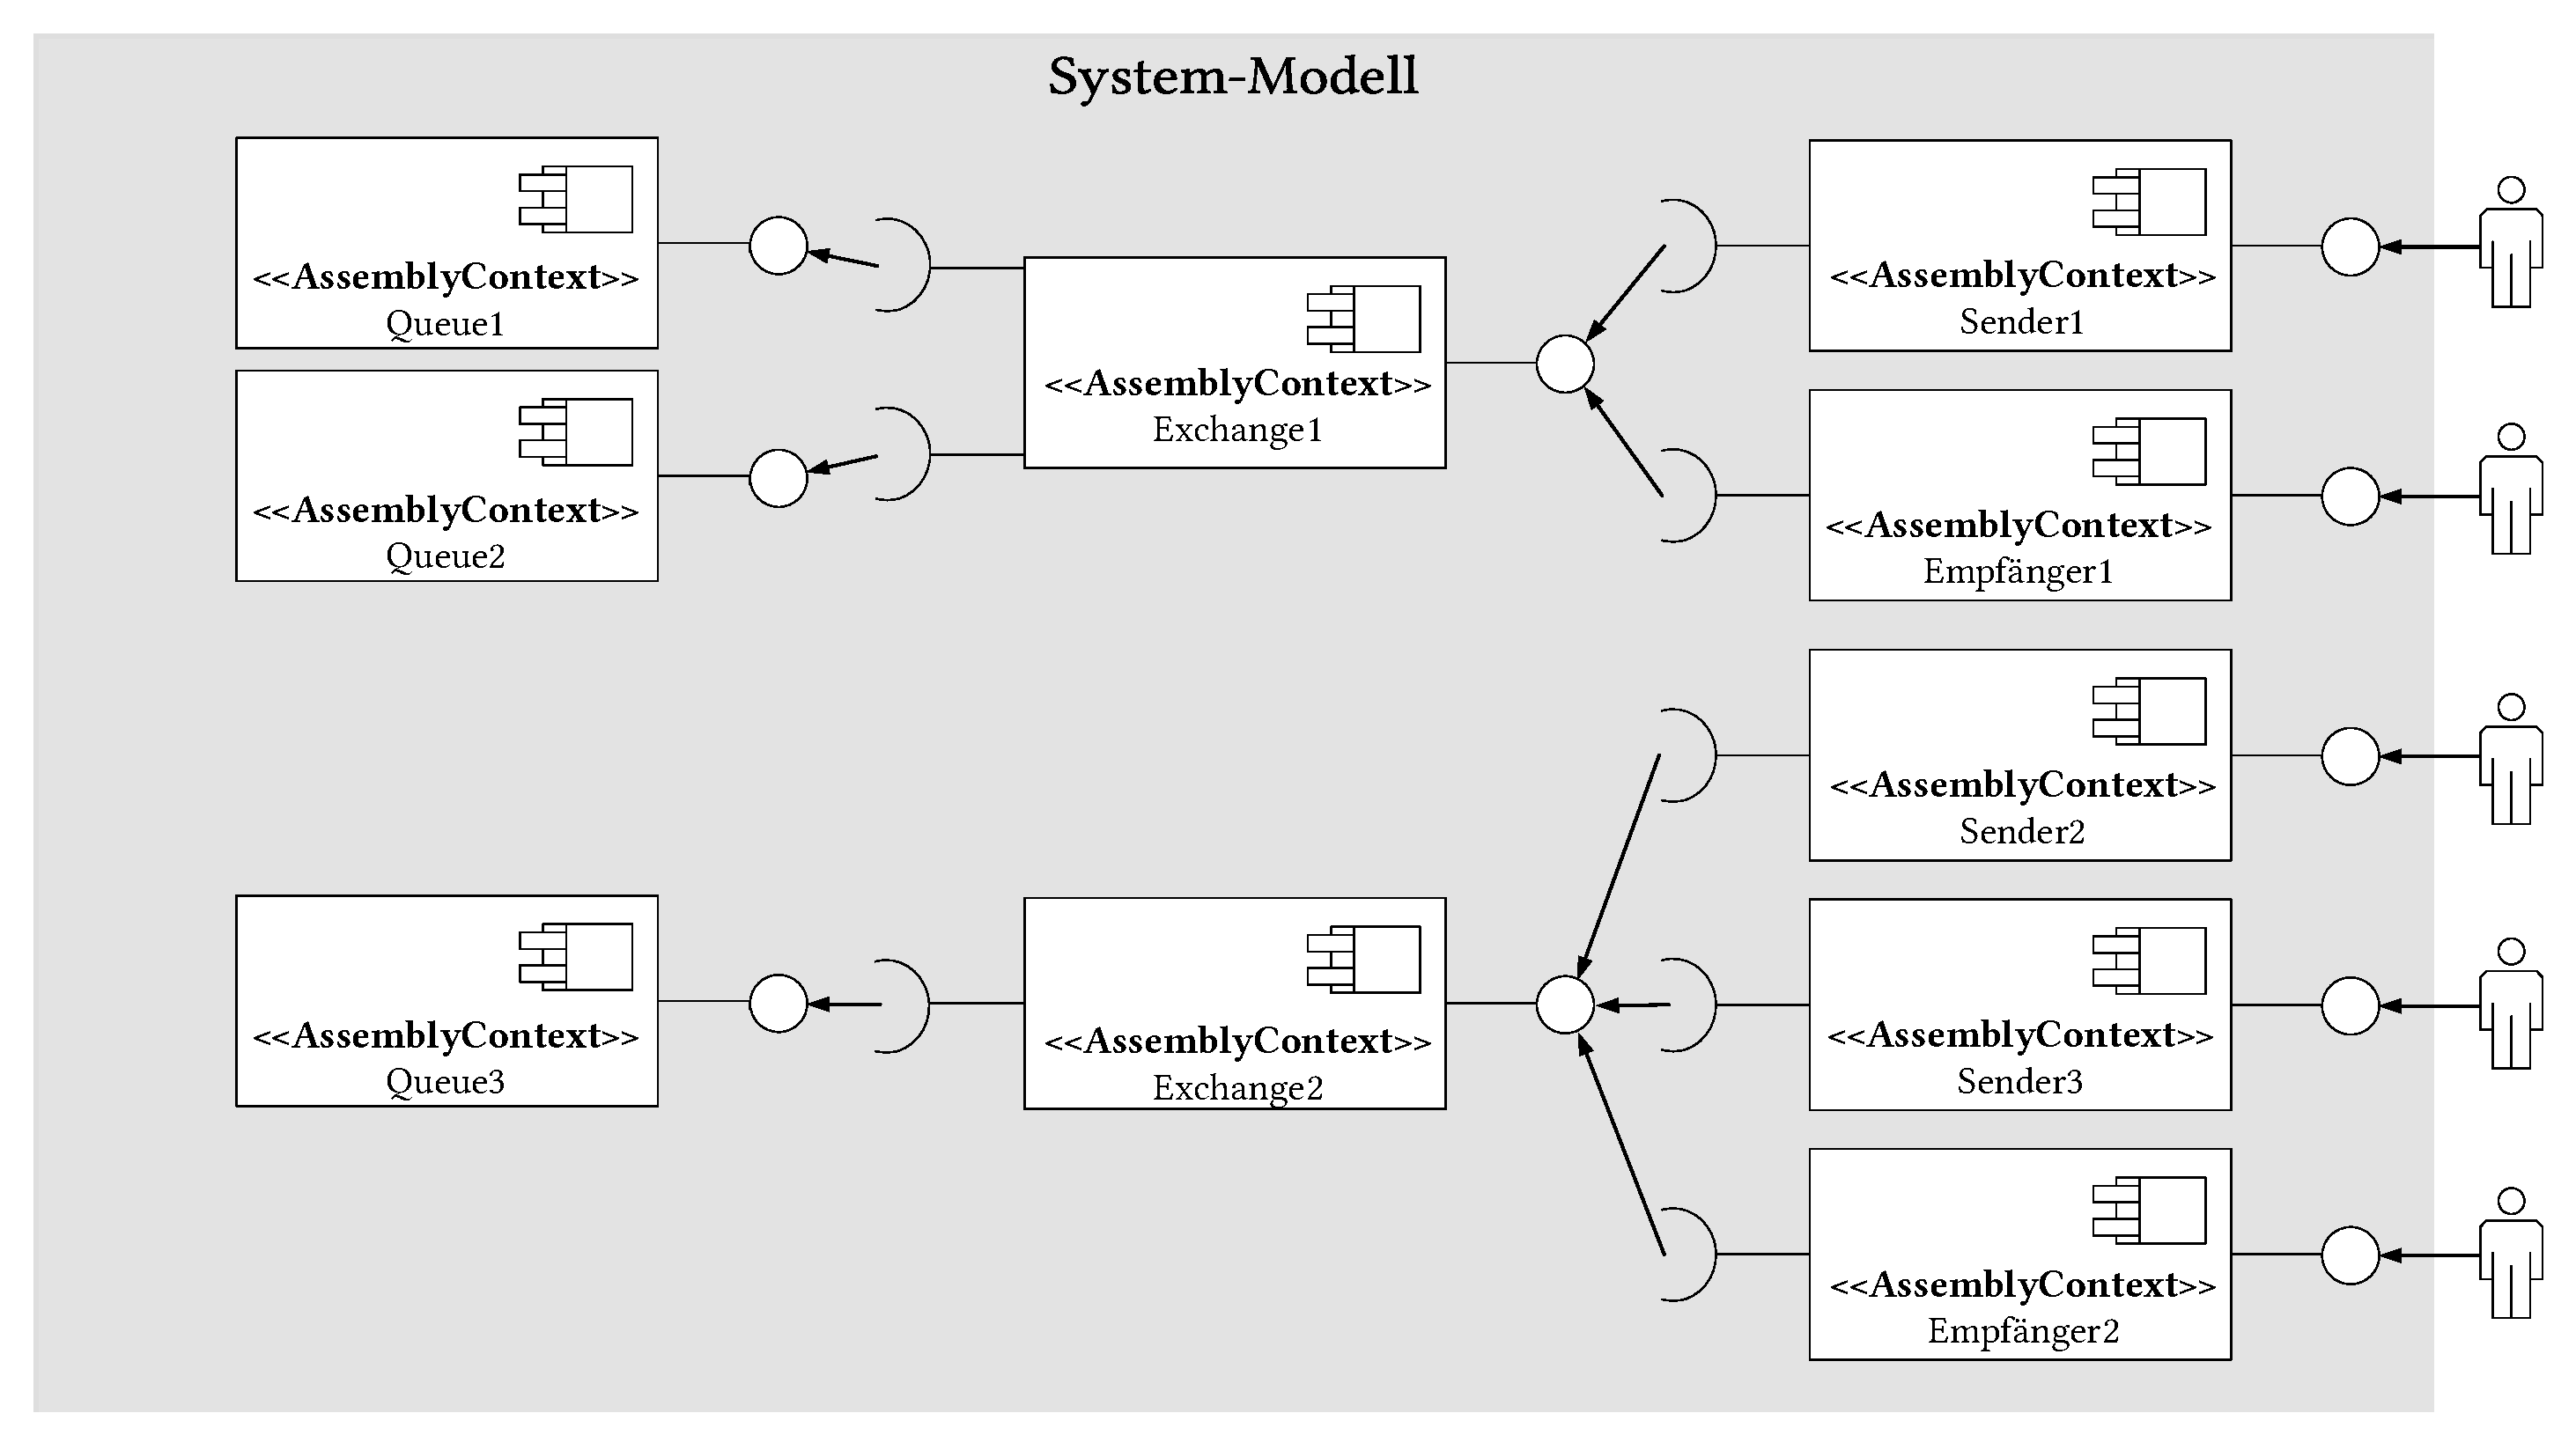
\includegraphics[width=1.4\textwidth, angle=90]{images/modelling/modelingSystem.pdf}
  \caption{Systemmodell einer MOM}
  \label{img:mom_system}
\end{figure}
\subsection{Ausführungsumgebung und Allokation}
Im Ausführungsumgebungs-Modell kann der Software-Verteilungs-Experte die Hardware-Knoten und Netzwerkverbindungen darstellen. Für die zuvor definierten Komponenten müssen nun Ressourcen, mithilfe von \emph{ResourceContainer}n, definiert werden. Dabei können die Exchange-, Warteschlangen-, Sender- und Empfänger-Komponente beliebig verteilt werden, wie auch bei einer tatsächlichen MOM. Dabei können mehrere Komponenten auf einem \emph{ResourceContainer} bereitgestellt werden. Dabei muss beachtet werden, dass der \emph{ResourceContainer} auf dem ein Exchange bereitgestellt ist mit den jeweiligen \emph{ResourceContainer} verbunden ist, auf dem die dazugehörigen Warteschlangen-, Sender- und Empfänger-Komponenten bereitgestellt sind. In \autoref{img:mom_ressorceEnv} ist eine mögliche Ausführungsumgebung für das oben beschriebene System dargestellt. Die einzelnen Komponenten sind auf dem jeweiligen \emph{ResourceContainer} mithilfe eines \emph{AllocationContext} bereitgestellt. Die Ausführungsumgebung besteht aus je einem MOM-\emph{ResourceContainer} für den jeweiligen Exchange und den an ihn angeschlossenen Warteschlangen. Die einzelnen Sender und Empfänger sind jeweils auf eigenen \emph{ResourceContainer}n verteilt und sind über \emph{LinkingResource}n mit der jeweiligen MOM-\emph{ResourceContainer} verbunden. 
\begin{figure}
\center
  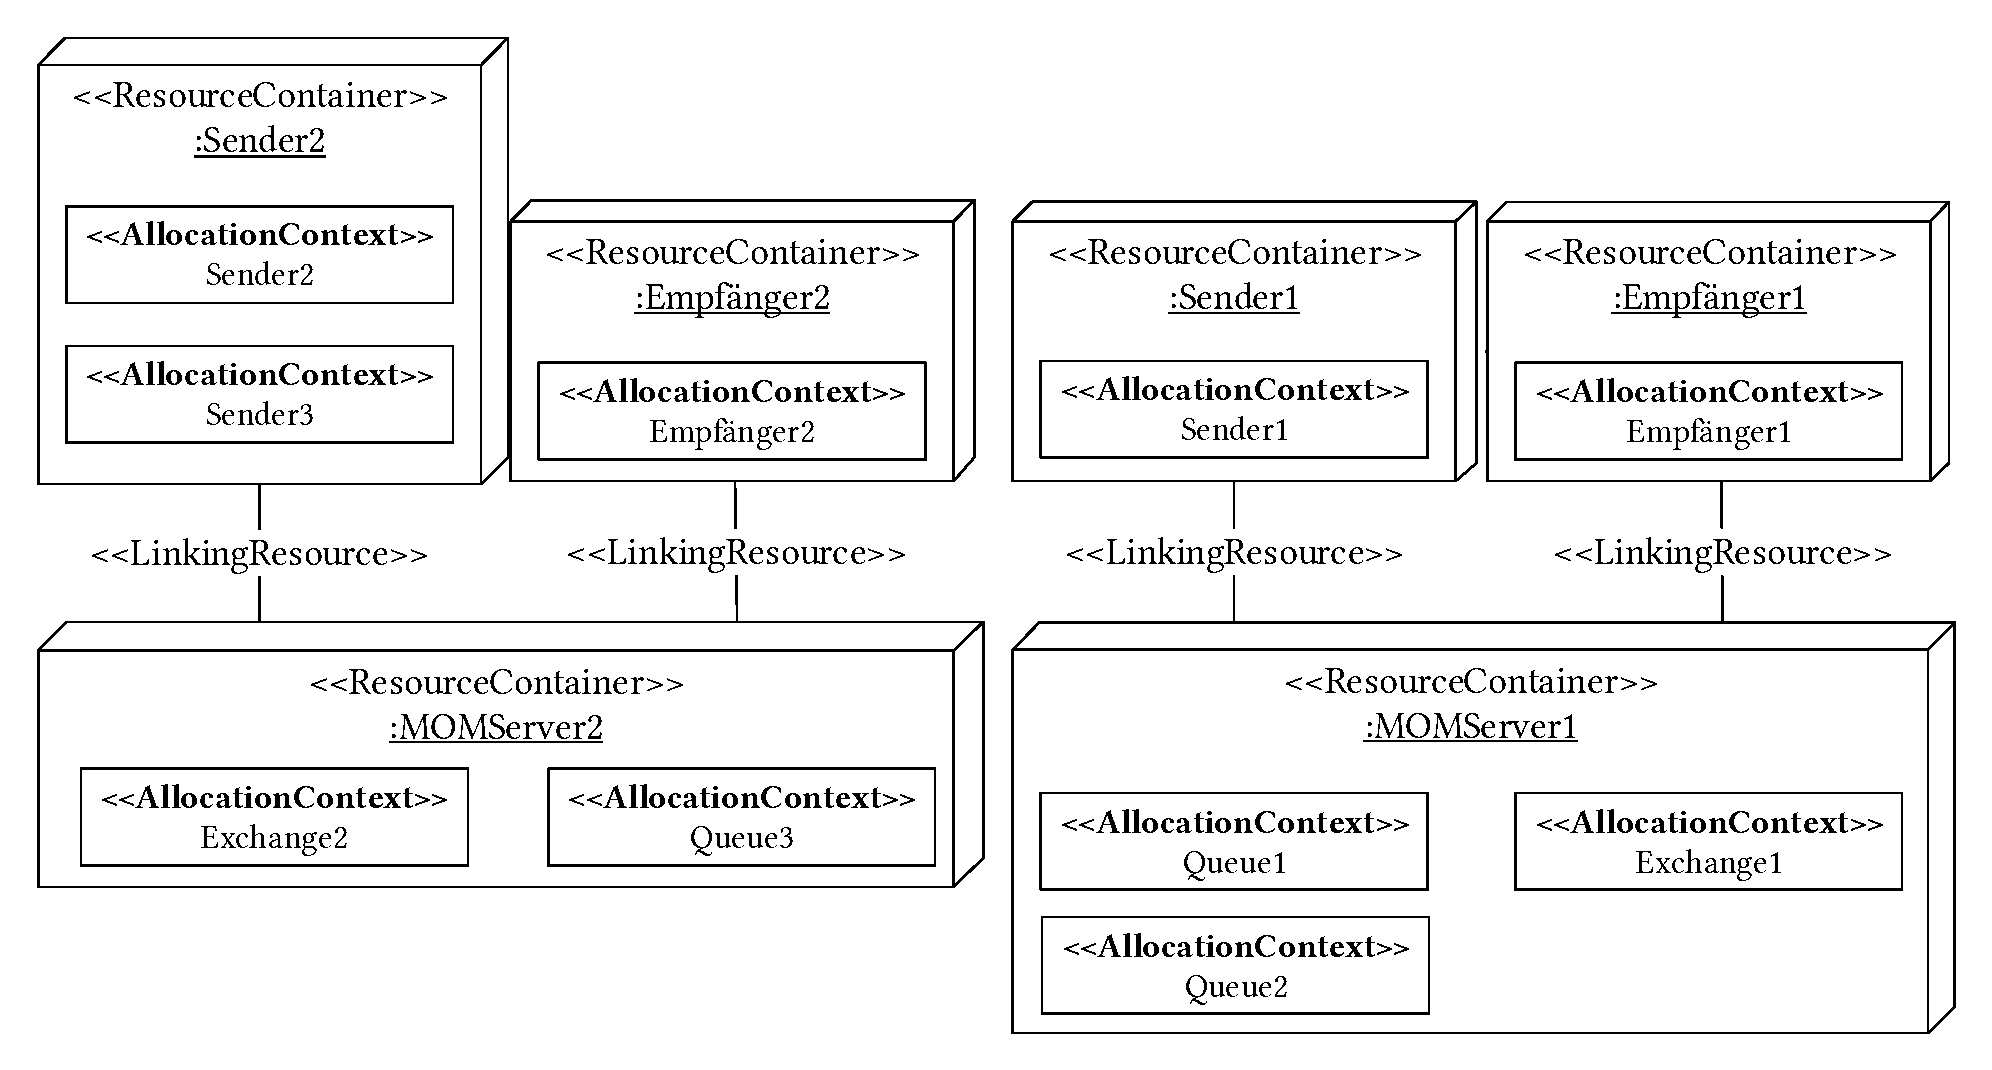
\includegraphics[width=1\textwidth]{images/modelling/modelingRecEnv.pdf}
  \caption{Ausführungsumgebung und Allokation einer MOM}
  \label{img:mom_ressorceEnv}
\end{figure}

\subsection{Nutzungsmodell}
Im Nutzungsmodell wird die Benutzung des Systems durch den Domänenexperten modelliert. Für jeden Sender und Empfänger wird dazu je ein \emph{UsageScenario} angelegt. Dieses beinhaltet das Verhalten eines Benutzers oder eines anderen Systems und seine Ankunftszeit (\emph{ArrivalTime}). Der Domänenexperte kann somit festlegen wie oft ein Sender oder Empfänger pro Zeiteinheit ankommt, um Nachrichten zu senden oder zu empfangen. Außerdem kann dadurch die Anzahl der Nachrichten, die pro Zeiteinheit gesendet werden, abgebildet werden. Wenn zum Beispiel ein Sender pro 0,1 mal Zeiteinheit ankommt, heißt das, dass er 10 mal pro Zeiteinheit ankommt und somit 10 Nachrichten, pro Zeiteinheit, versendet. Neben der Ankunftzeit wird im \emph{UsageScenario} auch das Verhalten modelliert. Mithilfe eines \emph{EntryLevelSystemCall}s kann die passende Funktion im passenden Exchange aufgerufen werden. Möchte ein Sender eine Nachricht an einen Exchange senden, muss er mithilfe des \emph{EntryLevelSystemCall}s den passenden Exchange auswählen. Mithilfe von \emph{UsageVariable}n, können dem Aufruf außerdem Parameterbelegungen mitgegeben werden. Mithilfe dieses Mechanismus kann für jeden Aufruf spezifiziert werden, wie groß die Nachricht, die gesendet oder empfangen werden soll, ist und zu welcher Warteschlange oder Topic sie gehört. In \autoref{img:mom_usage} ist ein mögliches Nutzungsmodell, für einen Teil, des oben beschriebenen Systems dargestellt. Die beiden dargestellten \emph{UsageScenario}s senden und empfangen Nachrichten über Exchange1. Das \emph{ProducerScenario} stellt den Sender des Systems dar. Seine Interaktion mit dem System besteht darin, die \emph{distribute}-Funktion im Exchange1 aufzurufen und dabei eine Nachricht mit 5000 Bytes zu versenden. Da seine Ankunftszeit 0,1 beträgt, tut er dies zehn mal pro Zeiteinheit. Das \emph{ConsumerScenario} stellt den Empfänger des Systems dar. Seine Interaktion mit dem System besteht darin, die \emph{receive}-Funktion im Exchange1 aufzurufen und dabei eine Nachricht mit 5000 Bytes zu empfangen. Da seine Ankunftszeit 0,5 beträgt, tut er dies zwei mal pro Zeiteinheit. Der Empfänger entnimmt somit pro Zeiteinheit nur zwei der zehn Nachrichten aus der Warteschlange. Die restlichen bleiben in der Warteschlange und sorgen dafür, dass diese anwächst. Diese Modellierung geht davon aus, dass Senden und Empfangen von Nachrichten immer paarweise geschehen. Somit ist ein Abholen von mehreren Nachrichten auf einmal nicht vorgesehen.
\begin{figure}
\center
  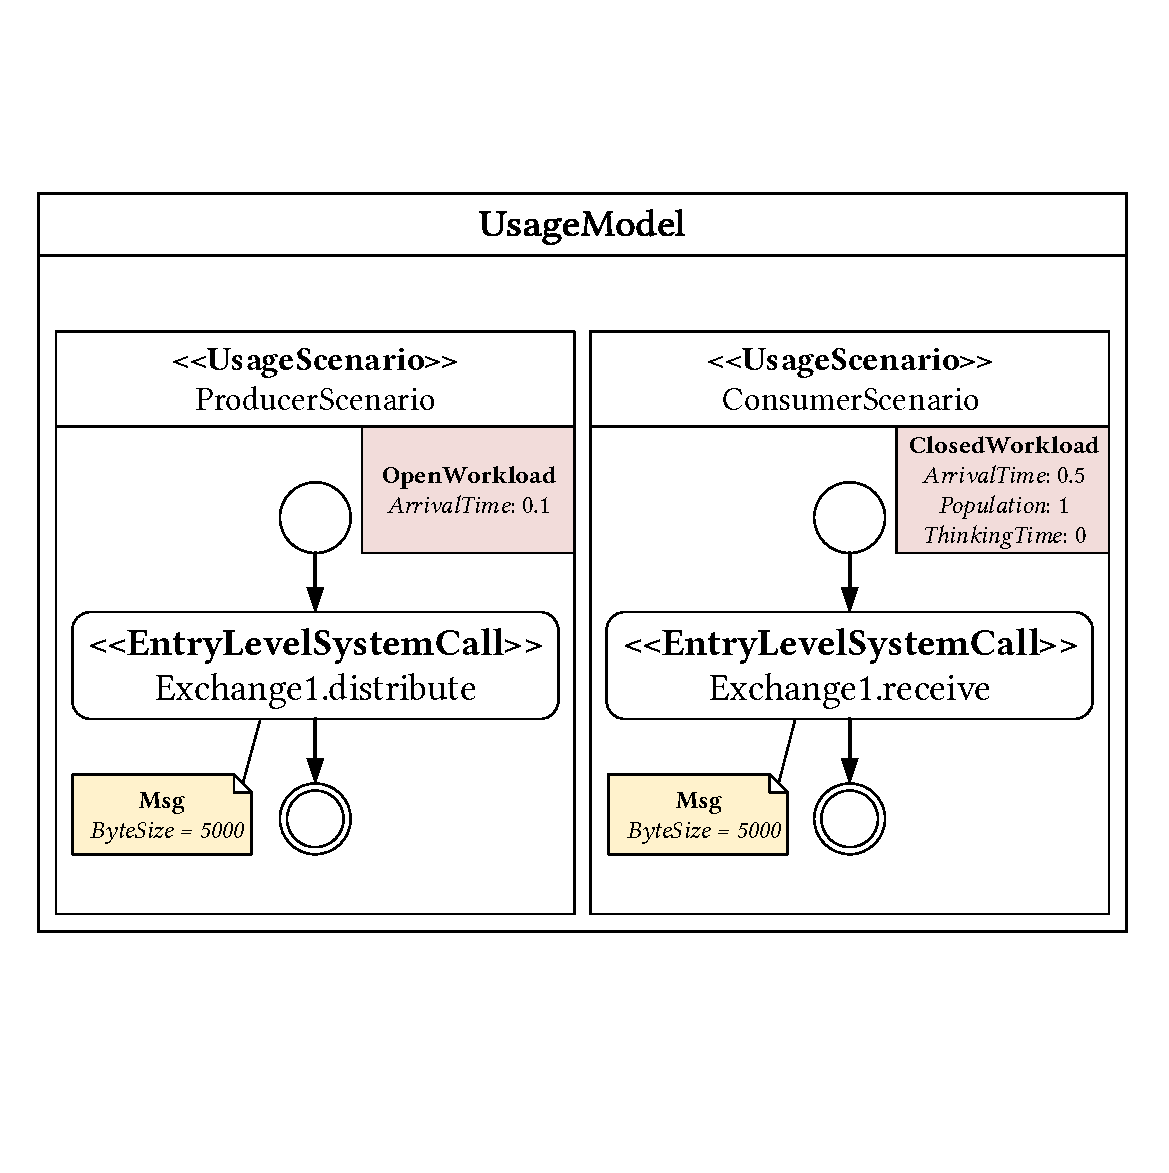
\includegraphics[width=1\textwidth]{images/modelling/modelingUsage.pdf}
  \caption{Nutzungsmodell einer MOM mit einem Sender und Empfänger}
  \label{img:mom_usage}
\end{figure}

\section{Modellkalibrierung}
\label{sec:rmqRd}
In \cite{palladio17} wird Modellkalibrierung als Anreicherung von Modellen mit quantitativen Daten, wie Ressourcenbedarf, beschrieben. Je nachdem wie weit entwickelt das System ist, können diese Daten mithilfe von verschiedenen Techniken gewonnen werden. Mithilfe von Application-Performance-Monitoring wurde in \autoref{sec:rmqBenchmark} RMQ ausgemessen und die Ergbnisse dort beschrieben. Im Folgenden sollen die Ergebnisse interpretiert und benutzt werden um die Modelle zu kalibrieren.
%Das Ziel ist, dass der Benutzer keinen MOM spezifischen RD angeben muss. \\

In \autoref{sec:oneMsgLatency} wurde die Latenz einer nicht-persistenten Nachricht mit verschiedenen Größen ausgemessen. Darin ist ein lineares Wachstum der Latenz mit Ansteigen der Nachrichtengröße zu beobachten. Dies legt die Vermutung nahe, dass diese beiden Variablen voneinander abhängen. Um diese Vermutung zu bestätigen wurde für die Variablen Latenz und Nachrichtengröße die Korrelation berechnet. Dabei ist die Korrelation ein statistisches Maß, das den Grad der linearen Abhängigkeit zwischen zwei Variablen anzeigt, die im Paar auftreten. Ist diese Abhängigkeit hoch, liegt der Wert nahe eins. Liegt der Wert dagegen bei minus eins, besteht eine negative Korrelation, d.h. steigt Variable A, sinkt Variable B. Wenn der Wert nahe oder gleich null ist, besteht keine Abhängigkeit. Die Korrelation der Variablen Latenz und Nachrichtengröße ist 0,99. Somit ist eine hohe lineare Abhängigkeit der Variablen gezeigt. Als nächstes soll mithilfe einer linearen Regressionsanalyse ein Ressourcenbedarf für das Modell definiert werden. Das Ziel einer linearen Regressionsanalyse ist es, eine lineare Beziehung zwischen einer Prädiktorvariable Y und der Reaktionsvariable X herzustellen, so dass der Wert von X geschätzt werden kann, wenn nur der Wert des Prädiktoren Y bekannt ist. Die dabei entstandene Regressionsgerade hat die Form: \[Latenz = 1256,2782902 + (0,003299 * Nachrichtengr.)\] und ist in \autoref{img:regplot} eingezeichnet. Da bei der Messung Sender und Empfänger nicht getrennt ausgemessen werden konnten, soll dieser Term als Ressourcenbedarf einer Nachricht dienen, sobald diese aus der Warteschlange entnommen wird. Dabei wird die Annahme getroffen, dass der Ressourcenbedarf in der jeweiligen Warteschlange anfällt, sobald die Nachricht aus ihr entnommen wird. 
\begin{figure}
\center
  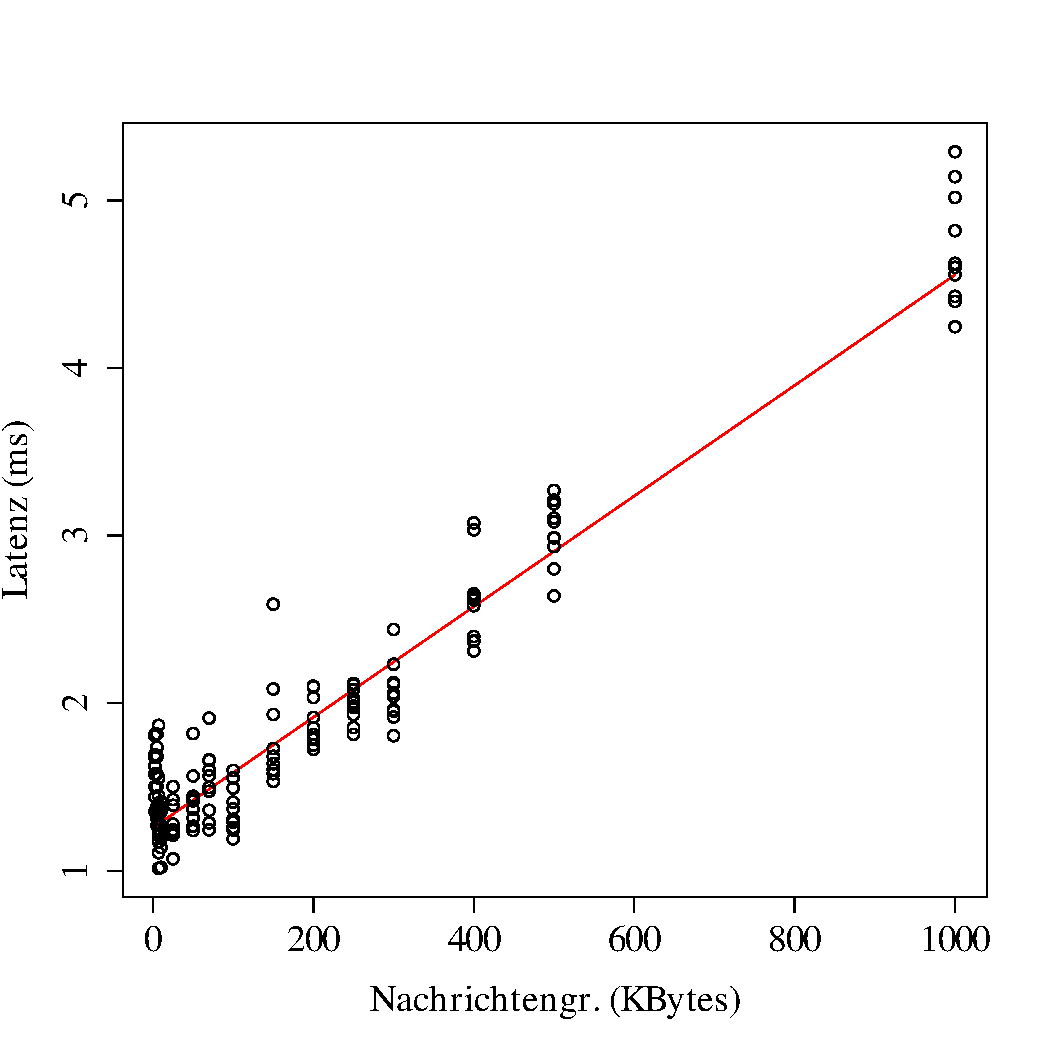
\includegraphics[width=0.7\textwidth]{images/modelling/oneMsgRegression.pdf}
  \caption{Messpunkte und die Regressionsgerade aus der Regressionsanalyse für nicht-persistente Nachrichten}
  \label{img:regplot}
\end{figure}

\par
Neben nicht-persistenten Nachrichten wurden auch persistente Nachrichten und die Konfiguration für Lazy-Warteschlangen ausgemessen. Im Folgenden betrachten wir den Fall der persistenten Nachrichten. Auch hier wurde wie oben beschrieben zunächst die Korrelation der beiden Variablen, Nachrichtengröße und Latenz, berechnet. Mit 0,995 ist diese ebenfalls sehr hoch. Die entstandene Regressionsgerade hat die Form: \[Latenz = 2082,691737 + (0,004737 * Nachrichtengr.)\] und ist in \autoref{img:regplotpersistent} eingezeichnet. Dieser Term soll nun als Ressourcenbedarf einer Nachricht dienen, sobald diese aus der Warteschlange entnommen wird, wenn persistente Nachrichten betrachtet werden sollen.
\begin{figure}
\center
  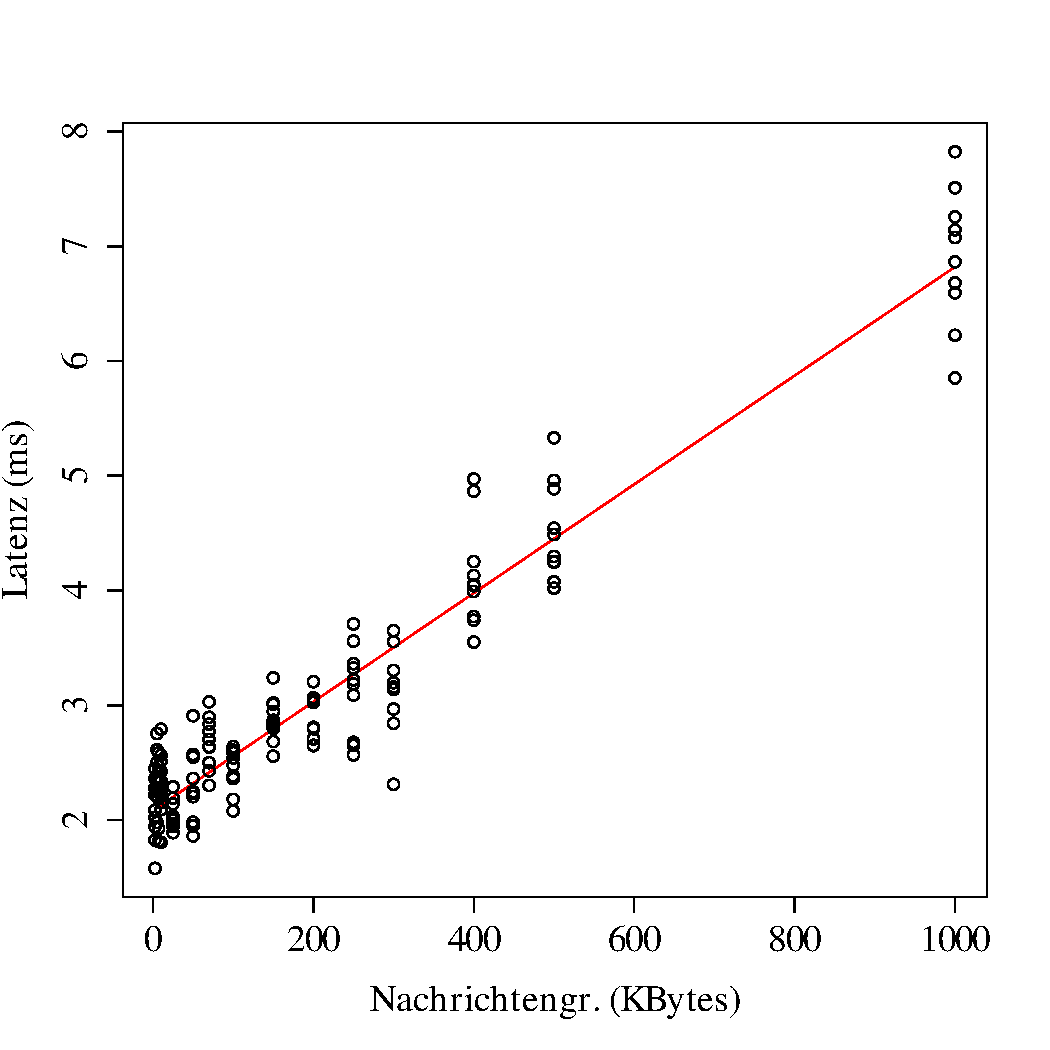
\includegraphics[width=0.7\textwidth]{images/modelling/persistentRegression.pdf}
  \caption{Messpunkte und die Regressionsgerade aus der Regressionsanalyse für persistente Nachrichten}
  \label{img:regplotpersistent}
\end{figure}

Als nächstes wird die Konfiguration für Lazy-Warteschlangen betrachtet. Die Korrelation der beiden Variablen, Nachrichtengröße und Latenz, ist mit 0,995 ebenfalls sehr hoch. Die entstandene Regressionsgerade hat die Form: \[Latenz = 1602,5021193 + (0,0049697 * Nachrichtengr.)\] und ist in \autoref{img:regplotlazy} eingezeichnet. Dieser Term soll nun als Ressourcenbedarf einer Nachricht dienen, sobald diese aus der Warteschlange entnommen wird, wenn Lazy-Warteschlangen betrachtet werden sollen.
\begin{figure}
\center
  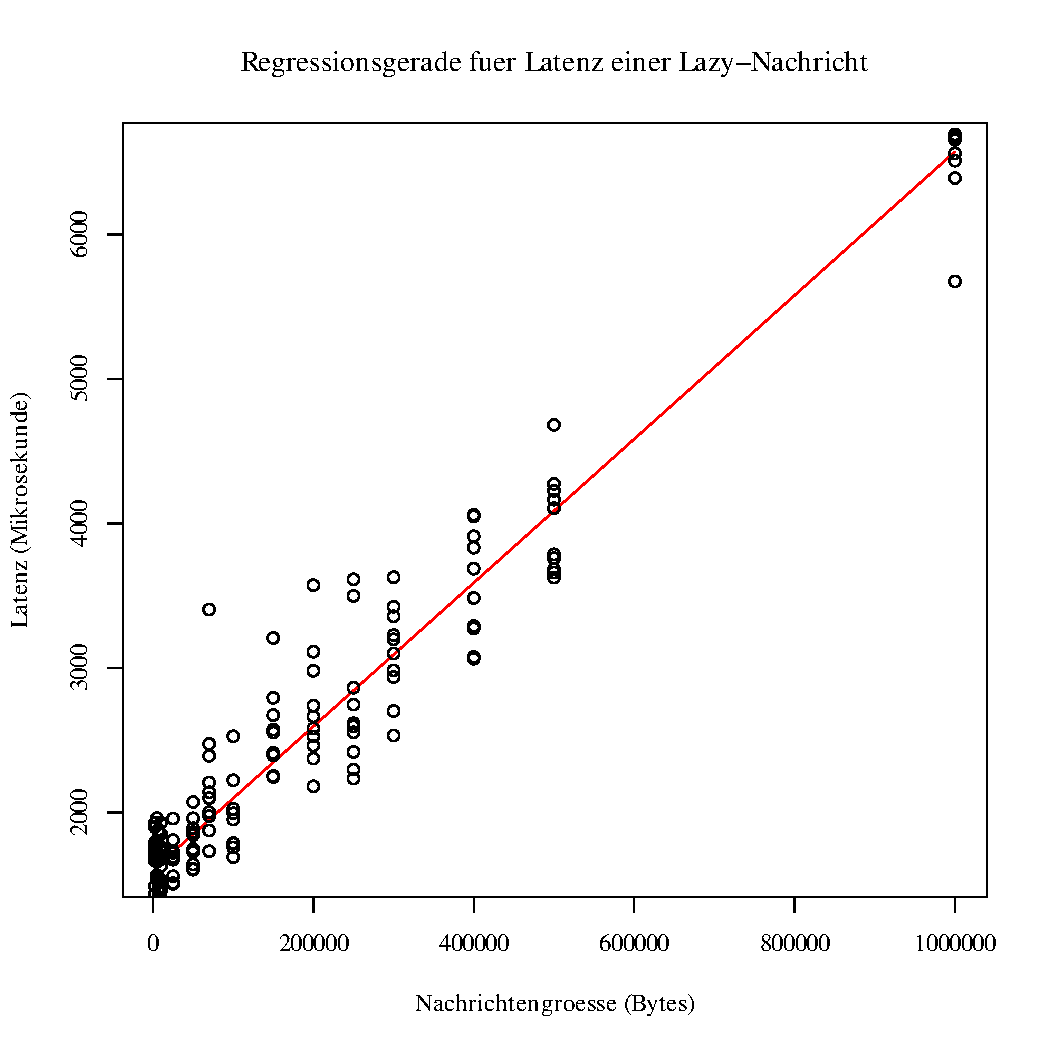
\includegraphics[width=0.7\textwidth]{images/modelling/oneMsgLazyRegression.pdf}
  \caption{Messpunkte und die Regressionsgerade aus der Regressionsanalyse für Lazy-Warteschlangen.}
  \label{img:regplotlazy}
\end{figure}

In \autoref{sec:maxthroughput} wurde gemessen, was der mögliche Datendurchsatz ist. Dabei wurde eine Messung mit und ohne Empfänger durchgeführt. Der Maximalwert aus der Messung ohne Empfänger wird in die \emph{distribute}-Funktion und der Maximalwert aus der Messung mit Empfänger wird in die \emph{receive}-Funktion, des jeweiligen Exchange eingetragen. Der Ressourcenbedarf hat dabei die Form \[Nachrichtengr. /  Durchsatz\]. 
Auch die Netzwerklatenz, die in \autoref{sec:oneMsgLatency} ausgemessen wurde, hat einen Einfluss auf die Latenz einer Nachricht. Wenn diese in der Modellierung betrachtet werden soll, kann diese in den jeweiligen Exchange eingetragen werden. Beide Ressourcenanforderungen werden dabei als Delay-Ressource in die jeweilige Exchange-Komponenten eingetragen, da die Annahme getroffen wird, dass diese Ressourcenanforderungen im MOM-System auftreten. \par
Die zuvor beschriebenen Modelle können nun mithilfe der hier vorgestellten quantitativen Daten angereichert werden um eine Performance-Analyse zu ermöglichen. Im nächsten Schritt soll eine konkrete Modellierung vorgestellt werden, die mit den hier vorgestellten Daten angereichert wird. 

%Somit ergibt sich f die Response Time folgendes ergeben: Response Time: ByteSize / Throughput + RD / CPU + Latency + HddRD/HDD \\
%RD an Aquire um Latenz abzubilden

%Als erstes sollte die Sende und Empfangsrate abgebildet werden. Beobachtet man (ref zu Messung verschiedene Senderaten) bemerkt man fuer die ersten Messungen, solange Warteschlange nicht allzu voll wird, einen linearen Anstieg der Latenz. Daraus laesst sich zunaechst folgender RD ableiten:






%Latenz: Unter Latenz versteht man im MOM Kontext, die Zeit, die eine einzelne Nachricht braucht um beim Consumer anzukommen. Da jede Nachricht einen Zeitstempel bekommt kann die Zeit gemessen werden, wenn sie aus der Warteschlange entnommen wurde.

%welche Effekte koennen wir so hoffentlich abbilden

\section{Untersuchung der MOM Modellierung}
In den Abschnitten zuvor wurde vorgestellt wie die Modellierung eines Systems aussehen soll, die eine MOM zum Nachrichtenaustausch verwendet. Im Folgenden wird eine konkrete Modellierung vorgestellt, die mit den quantitativen Daten aus \autoref{sec:rmqRd} angereichert wird. Anschließend wird eine Performance-Analyse auf der Modellierung ausgeführt. Die Ergebnisse werden anschließend mit den Messungen aus \autoref{sec:rmqBenchmark} verglichen.

\subsection{Anwendungszenario}
Im Folgenden betrachten wir das in \autoref{img:simulationscenario} abgebildete Szenario. Darin befindet sich eine Sender und eine Empfänger-Komponente. Beide sind mit der Exchange-Komponente verbunden. Der Exchange ist genau mit einer Warteschlange verbunden. Diese ist entweder mit der Ressourcen Anforderung für eine Nachricht ohne oder mit Lazy-Warteschlangen angereichert. Die Exchange- und Warteschlangen-Komponente sind auf einem gemeinsamen MOM-ResourceContainer bereitgestellt. Die Sender- und Empfänger-Komponente sind jeweils auf einem eigenen ResourceContainer bereitgestellt. Der MOM-ResourceContainer ist jeweils mit dem Sender- und der Empfänger-ResourceContainer mithilfe einer LinkingResource verbunden. Je nachdem welches Szenario betrachtet wird, hat die Exchange-Komponenten die passende Ressourcen Anforderung für Durchsatz und Latenz eingetragen. Schließlich sind für den Sender und Empfänger jeweils ein UsageScenario spezifiziert. Darin sind die jeweiligen Ankunftszeiten und Nachrichtengrößen modelliert.
% Der Sender sendet pro Zeiteinheit und der Empfaenger empfaengt pro Zeiteinheit eine bestimmte Menge an verschieden Großen Nachrichten. 
\begin{figure}
\center
  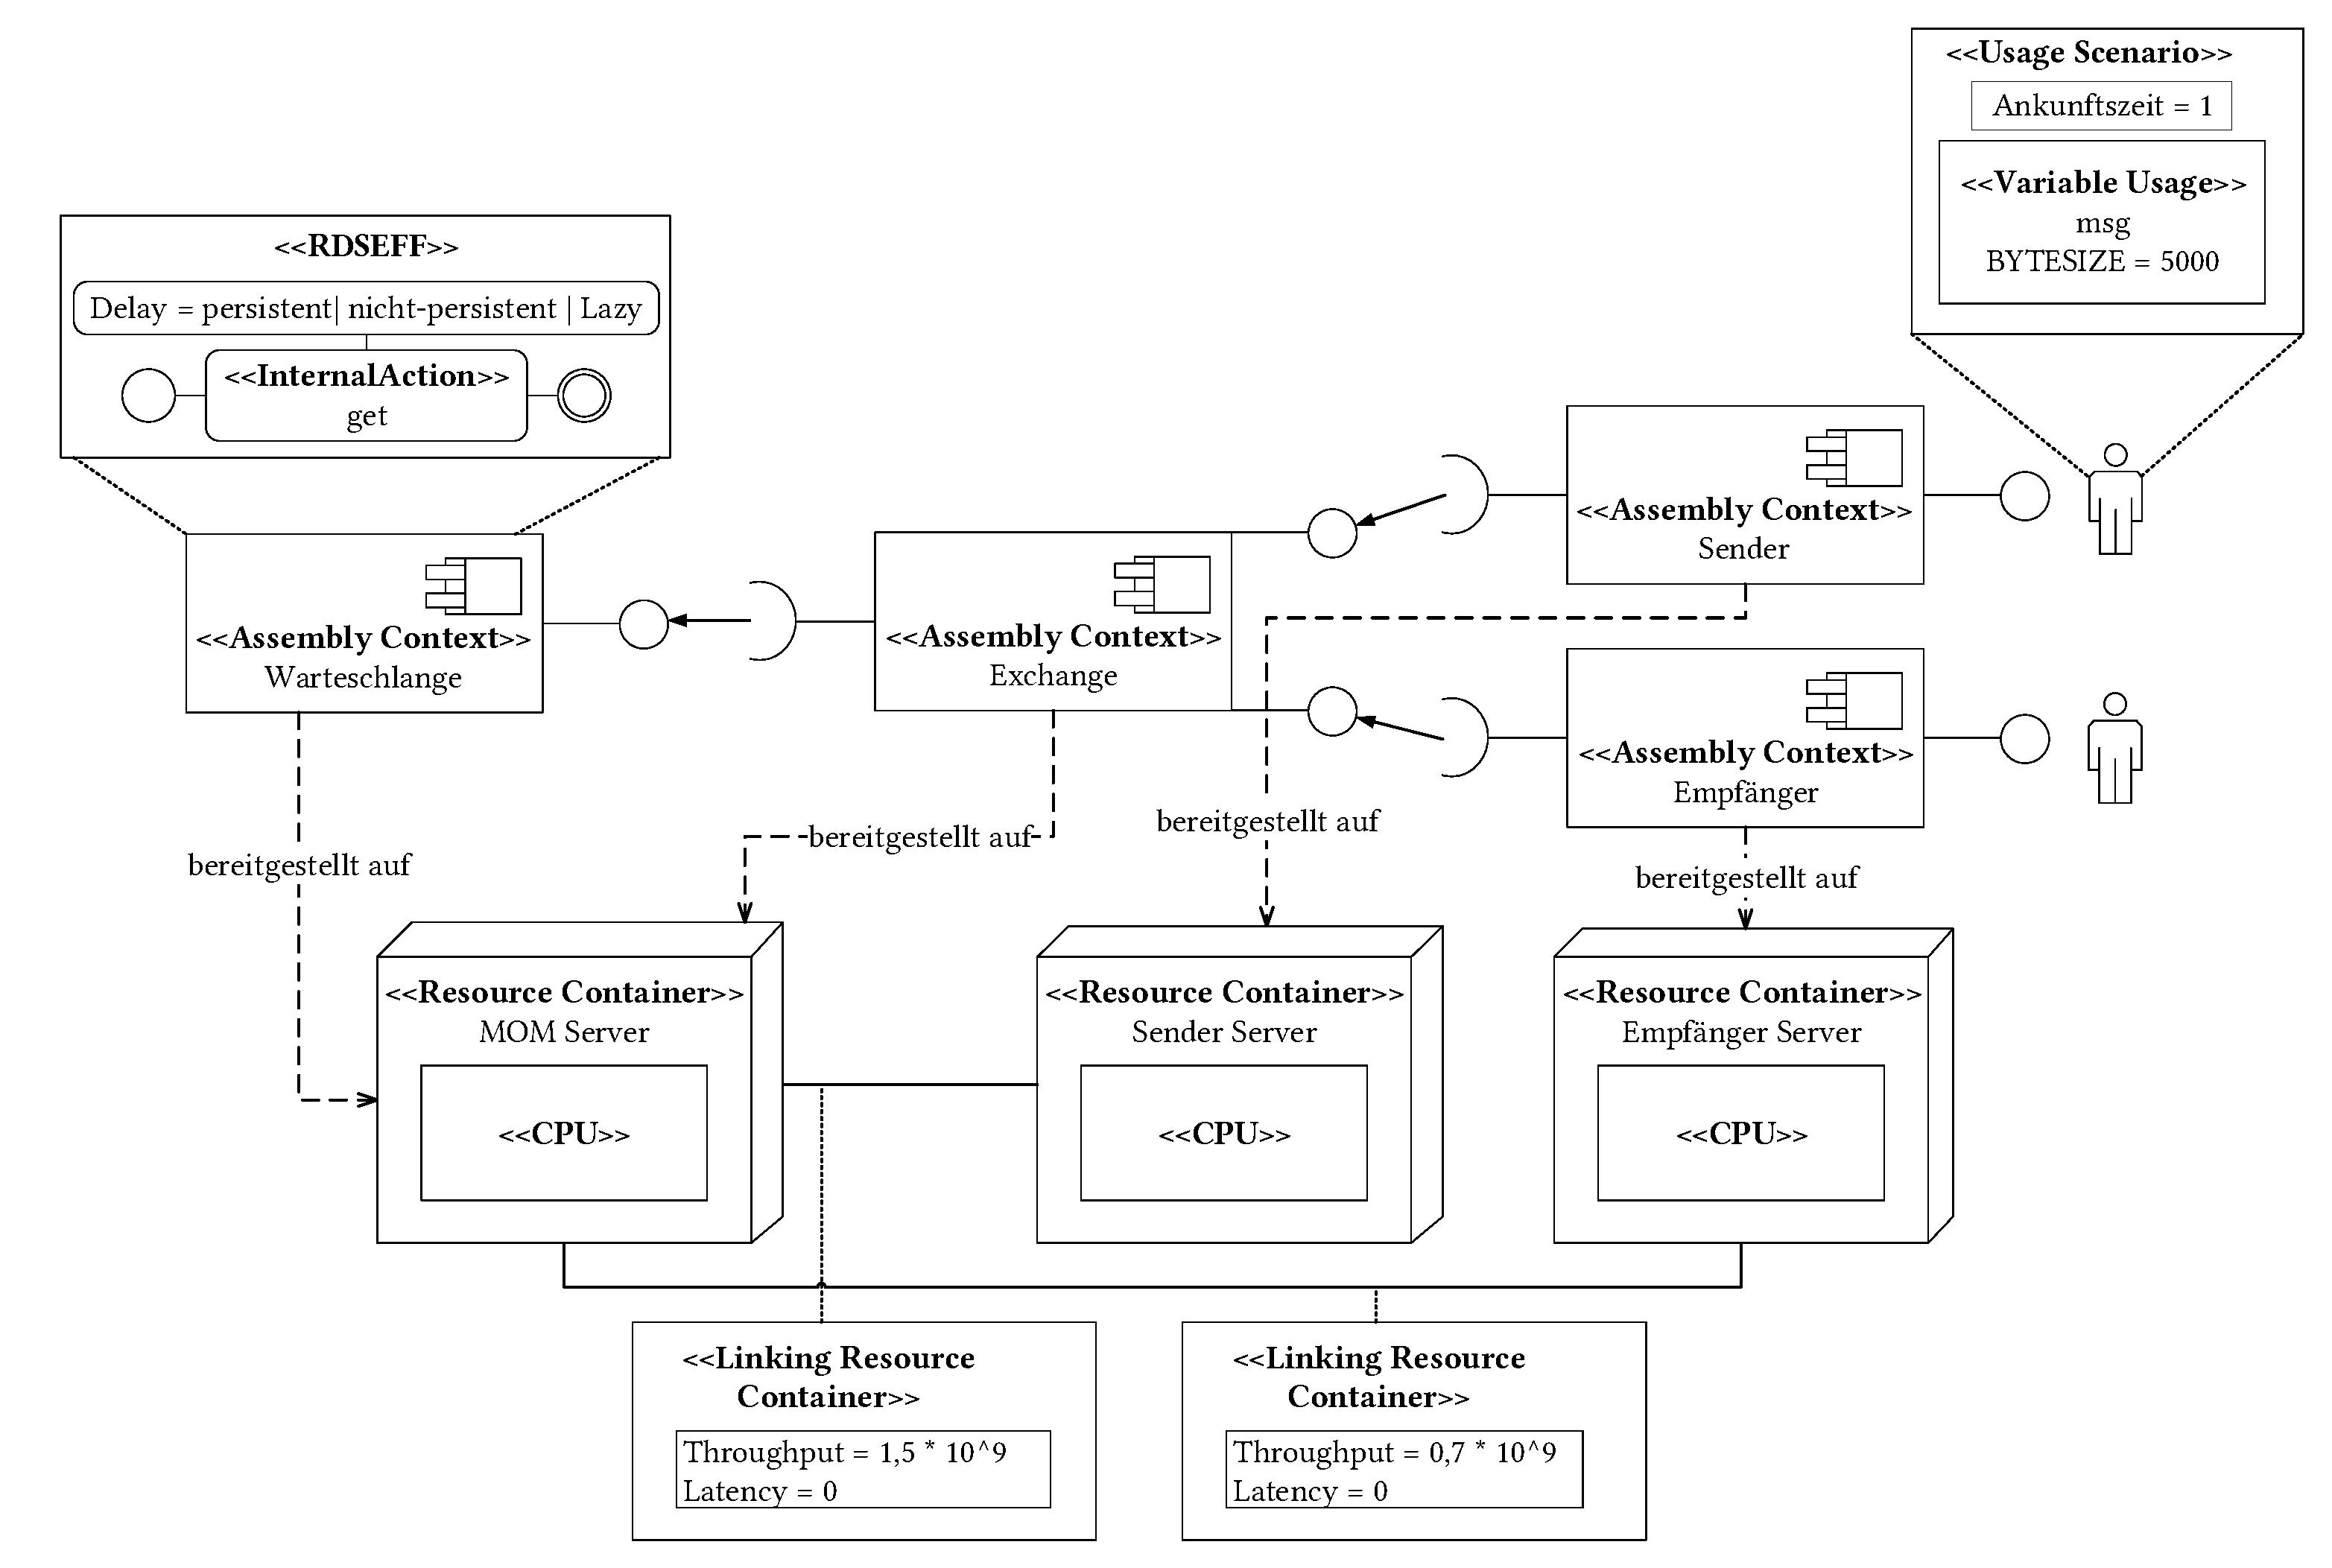
\includegraphics[width=1.35\textwidth, angle=90]{images/modelling/modelingSimulationSzenario.pdf}
  \caption{Auszug des Simulationsszenarios.}
  \label{img:simulationscenario}
\end{figure}
Im Folgenden wird diese Modellierung in einer Performance-Analyse eingesetzt.


\subsection{Performance-Analyse}
\label{sec:performanceanalyse}
Die Palladio-Bench bietet eine Sammlung von Qualitätsanalysen mit Hauptfokus auf Performance an. Nachdem in den vergangen Abschnitten eine MOM Modellierung und ihre Kalibrierung beschrieben wurde, kann im nächsten Schritt eine Performance-Analyse ausgeführt werden. Dazu wird das Analysewerkzeug \textbf{SimuCom} verwendet, das verschiedene Performance-Charakteristiken, darunter Antwortzeiten für Systeme und Komponenten, sowie die Auslastung einzelner Ressourcen berechnet. Im Folgenden werden die Ergebnisse der Performance-Analyse präsentiert und mit den Messungen aus \autoref{sec:rmqBenchmark} verglichen. Dazu wird für jede Simulation der Fehler zwischen dem gemessenen Wert und dem vom Modell vorhergesagten Wert berechnet. Dazu wird die folgende Formel verwendet: \[ Fehler\% = \frac{|Vorgersage - Messung|}{Messung} * 100 \] Für \textit{Vorgersage} wird der Wert aus der Modell-Vorhersage eingesetzt. Für \textit{Messung} wird der jeweilige Median aus den Messungen eingesetzt.
\subsubsection{Simulation 1} 
\label{sec:rmqSimulation1}
In der ersten Simulation wird der Fall betrachtet, dass Sender und Empfänger die gleichen Ankunftszeiten haben. Die gesendete Nachrichten haben die Größen 100, 200, 300, 400, 500 und 1000 Kbyte. Es handelt sich dabei um nicht-persistenten Nachrichten. Verglichen wurde mit den Messungen aus \autoref{sec:oneMsgLatency}. Der Sender, Empfänger und der Broker befinden sich jeweils auf der selben Maschine. Betrachtet wurden der Füllstand der Warteschlange und die Latenz der Nachrichten. 
%B
Da die Ankunftszeiten der beiden Akteure gleich sind, bleibt die Warteschlange die ganze Zeit über leer. Die Ergebnisse der Latenz einer Nachricht sind in \autoref{img:simulation1} abgebildet. Eingezeichnet sind dabei die Messpunkte der Messungen und die Ergebnisse der Simulation. In \autoref{tab:sim1} ist der Fehler für jede Größe angegeben. Dabei ist zu sehen, dass bei dieser Simulation der Fehler zwischen 19.98 \% und 30.67\% liegt.

\begin{figure}
\center
  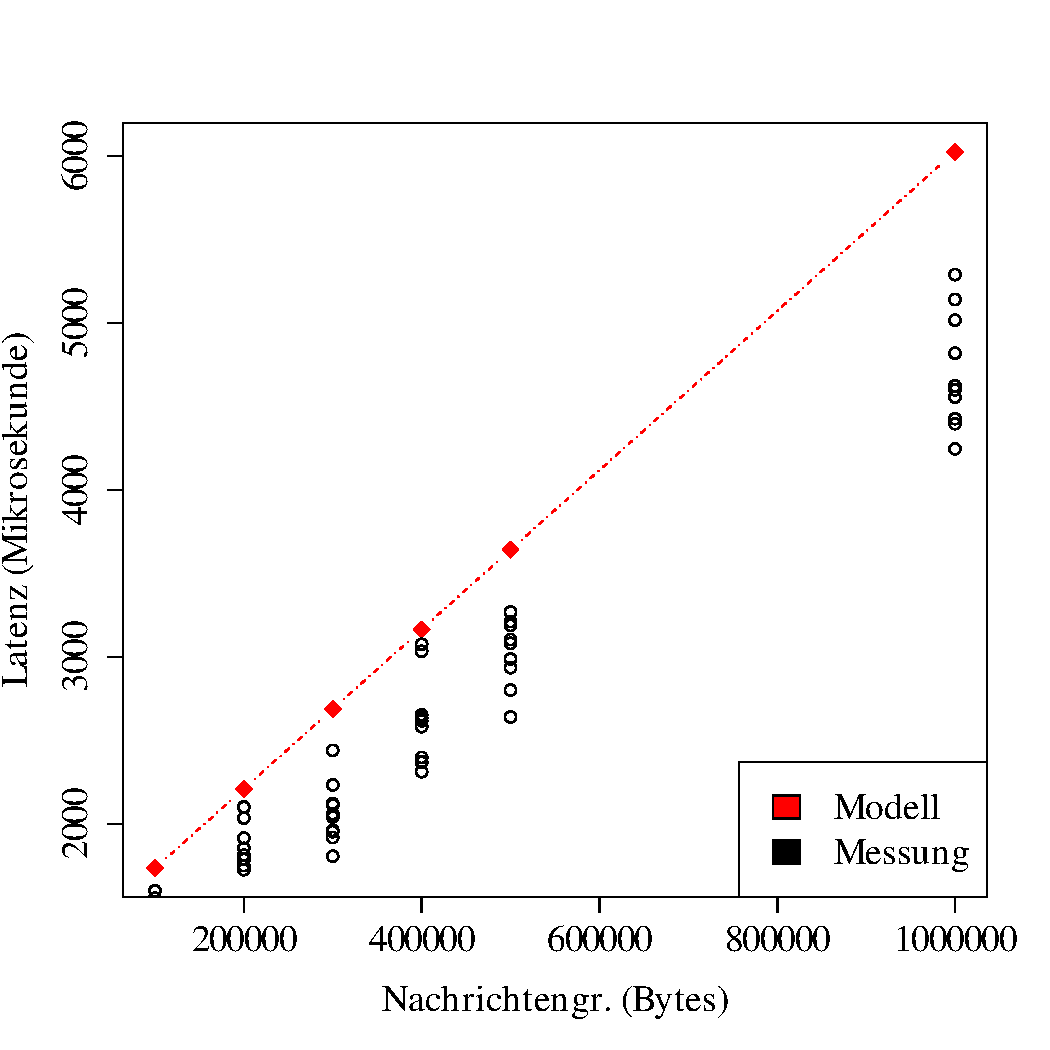
\includegraphics[width=0.7\textwidth]{images/modelSimulationResults/simulation1.pdf}
  \caption{Messung und Vorhersage der Latenz einer nicht-persistenten Nachricht mit verschiedenen Größen.}
  \label{img:simulation1}
\end{figure}

\begin{table}
  \begin{tabular}{| l | l | l | l |l | l | l |}
    \hline
    Nachrichtengröße (KB) & 100 & 200 & 300 & 400 & 500 & 1000 \\ \hline
    Messung (\mu s) & 1339 & 1833 & 2050,5 & 2599,5 & 3035 & 4612\\ \hline
    Vorhersage (\mu s) & 1733,3 & 2210,3 & 2687,3 & 3164,3 & 3641,4 & 6026,5\\ \hline
    Fehler (\%) & 29,45 & 20,58 & 31,06 & 21,73 & 19,98 & 30,67\\ \hline
    
    \hline
      \end{tabular}
	\caption{\label{tab:sim1} Fehler in \% zwischen Messung und Vorhersage für Simulation 1}
\end{table}





\subsubsection{Simulation 2} 
Diese Simulation betrachtet zusätzlich zu dem Fall aus Simulation 1 die Netzwerklatenz mit. Dazu sind Sender, Empfänger und Broker auf unterschiedlichen Maschinen. Die Nachrichten haben die größen 100, 200, 300, 400, 500 und 1000 Kbyte. Im Modell wurden für die LinkingRessources der Durchsatz und die Latenz, wie in \autoref{sec:rmqRd} beschrieben, für entfernte Broker angepasst. Die Messung mit der verglichen wurde ist in \autoref{sec:oneMsgLatency} beschrieben. Es wurden der Füllstand der Warteschlange und die Latenz der Nachrichten betrachtet. 
%B
Die Warteschlange bleibt über die Simulationsdauer leer, da die Ankunftszeiten der Sender und Empfänger gleich sind. Die Latenz der Nachrichten ist in \autoref{img:simulation2} abgebildet. Außerdem sind die Messpunkte aus der Messung eingetragen. In \autoref{tab:sim2} ist der Fehler für jede Größe angegeben. Der Fehler liegt zwischen 21.15\% und 33.43\%.
\begin{figure}
\center
  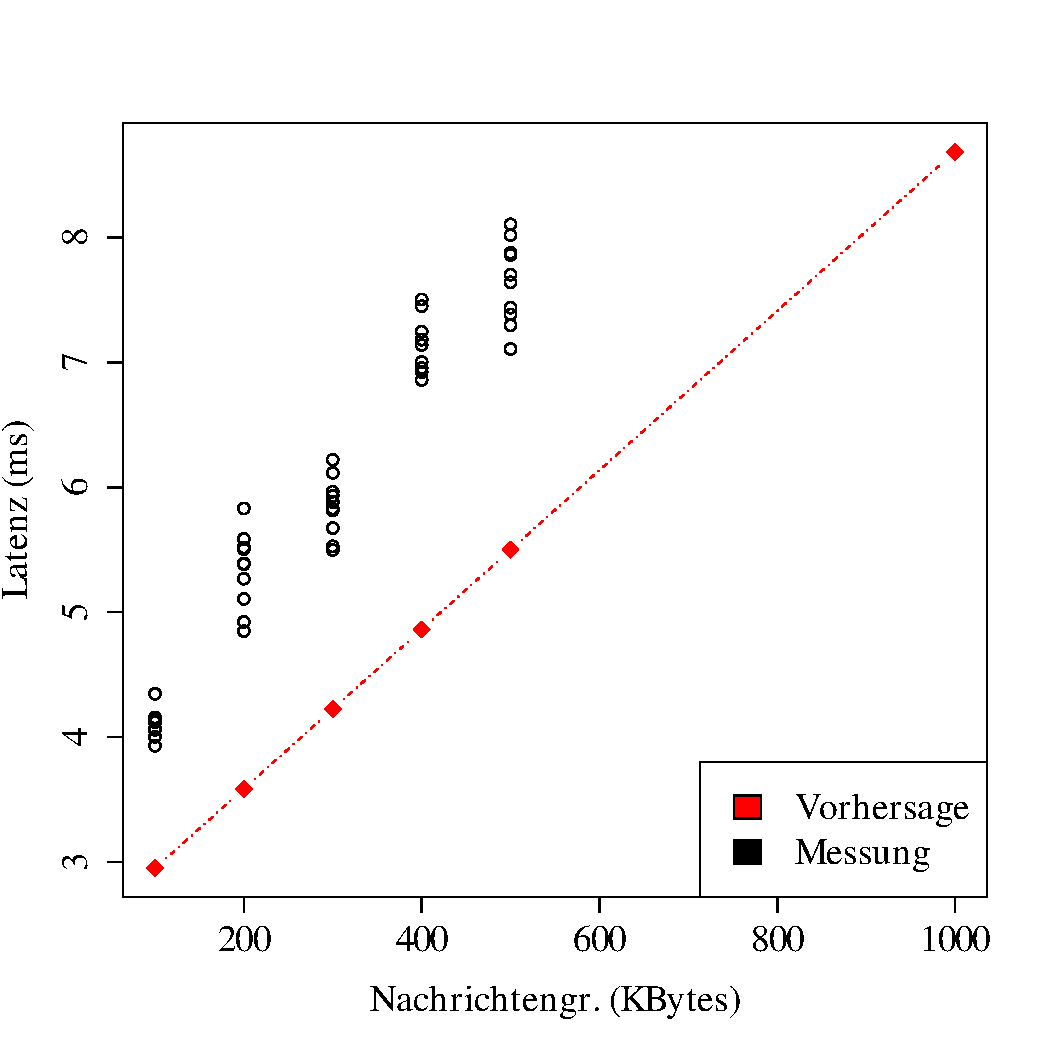
\includegraphics[width=0.7\textwidth]{images/modelSimulationResults/simulation2.pdf}
  \caption{Messung und Vorhersage der Latenz einer nicht-persistenten Nachricht, zu einem entfernten Broker, mit verschiedenen Größen.}
  \label{img:simulation2}
\end{figure}

\begin{table}
  \begin{tabular}{| l | l | l | l |l | l | l |}
    \hline
    Nachrichtengröße (KB) & 100 & 200 & 300 & 400 & 500 & 1000 \\ \hline
    Messung (\mu s) & 4093 & 5387,5 & 5856,5 & 7161 & 7672,5 & 11019\\ \hline
    Vorhersage (\mu s) & 2948,71 & 3586,41 & 4224,12 & 4861,83 & 5499,53 & 8688,07\\ \hline
    Fehler (\%) & 27,96 & 33,43 & 27,87 & 32,11 & 28,32 & 21,15\\ \hline
    
    \hline
      \end{tabular}
	\caption{\label{tab:sim2} Fehler in \% zwischen Messung und Vorhersage für Simulation 2}
\end{table}


\subsubsection{Simulation 3}
\label{sec:simulation3}
In dieser Simulation wird die Auswirkung der Ankunftszeiten auf das System geprüft. Verglichen wird mit der Messung aus \autoref{sec:queueGrowth}. Dabei ist die Ankunftszeit des Senders einmal pro Sekunde und die des Empfängers einmal alle zwei Sekunden. Der Füllstand der Warteschlange, sowie die Latenz der Nachrichten wird über die Zeit betrachtet.
%B
Die Ergebnisse sind in \autoref{img:simulation3} abgebildet. In \autoref{img:simulation3}a ist zu sehen, dass sich der Füllstand der Warteschlange bei Messung und Simulation gleich verhält und über die Zeit ansteigen, da jede Sekunde eine Nachricht in der Warteschlange unbearbeitet bleibt. In \autoref{img:simulation3}b sieht man außerdem die Auswirkungen auf die Latenz der einzelnen Nachrichten. Während bei der Messung die Latenz für die Nachrichten steigt, bleibt sie in der Modellierung unverändert. Dies liegt daran, dass die Latenz auch vom Füllstand der Warteschlange abhängt. In diesem Fall müsste der Füllstand bei der Berechnung der Latenz mit berücksichtigt werden. Dies ist mit SimuCom nicht möglich. 
\begin{figure}
\center
  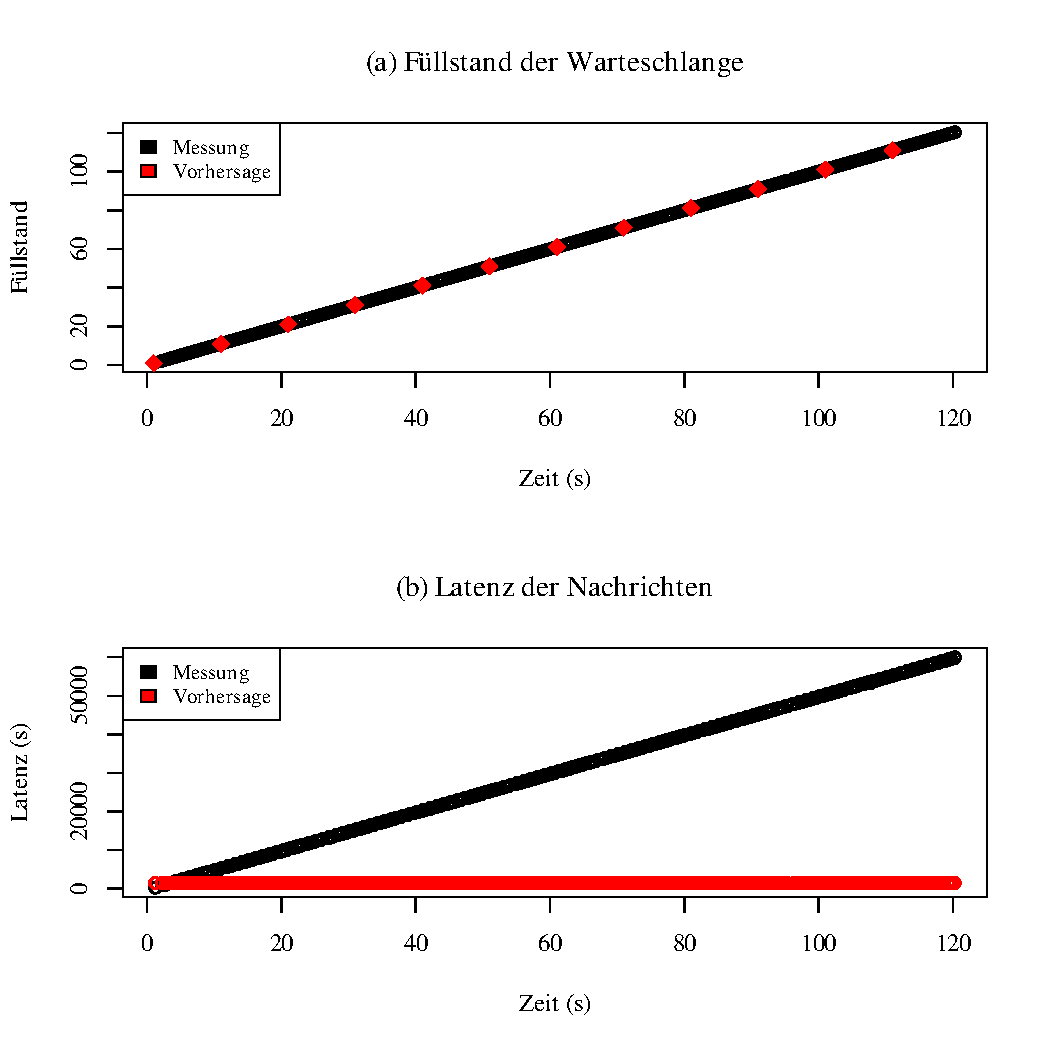
\includegraphics[width=0.7\textwidth]{images/modelSimulationResults/simulation3.pdf}
  \caption{Messung und Vorhersage des Anwachsen der Warteschlange.}
  \label{img:simulation3}
\end{figure}

\subsubsection{Simulation 4}
Mit dieser Simulation soll die Auswirkung mehrerer Empfänger auf das System überprüft werden. Die Frage dabei ist, ob mehrere Empfänger eine Warteschlange gemeinsam abarbeiten können und sich somit wie in der Messung aus \autoref{sec:varyingConsumer} verhalten. Im der folgenden Simulation ist die Ankunftszeit des Senders einmal pro Sekunde und die der beiden Empfänger jeweils einmal alle zwei Sekunden. Die Nachrichtengröße beträgt dabei, wie auch in der Messung, 10 KByte. Betrachtet werden der Füllstand der Warteschlange und die Latenz der einzelnen Nachrichten. 
%B
Die Simulation zeigt, dass beide Empfänger die Warteschlange gemeinsam abarbeiten können. Der Fehler zwischen Messung und Vorhersage der Latenz liegt bei 4.4\%. 

%\begin{figure}
%\center
 % 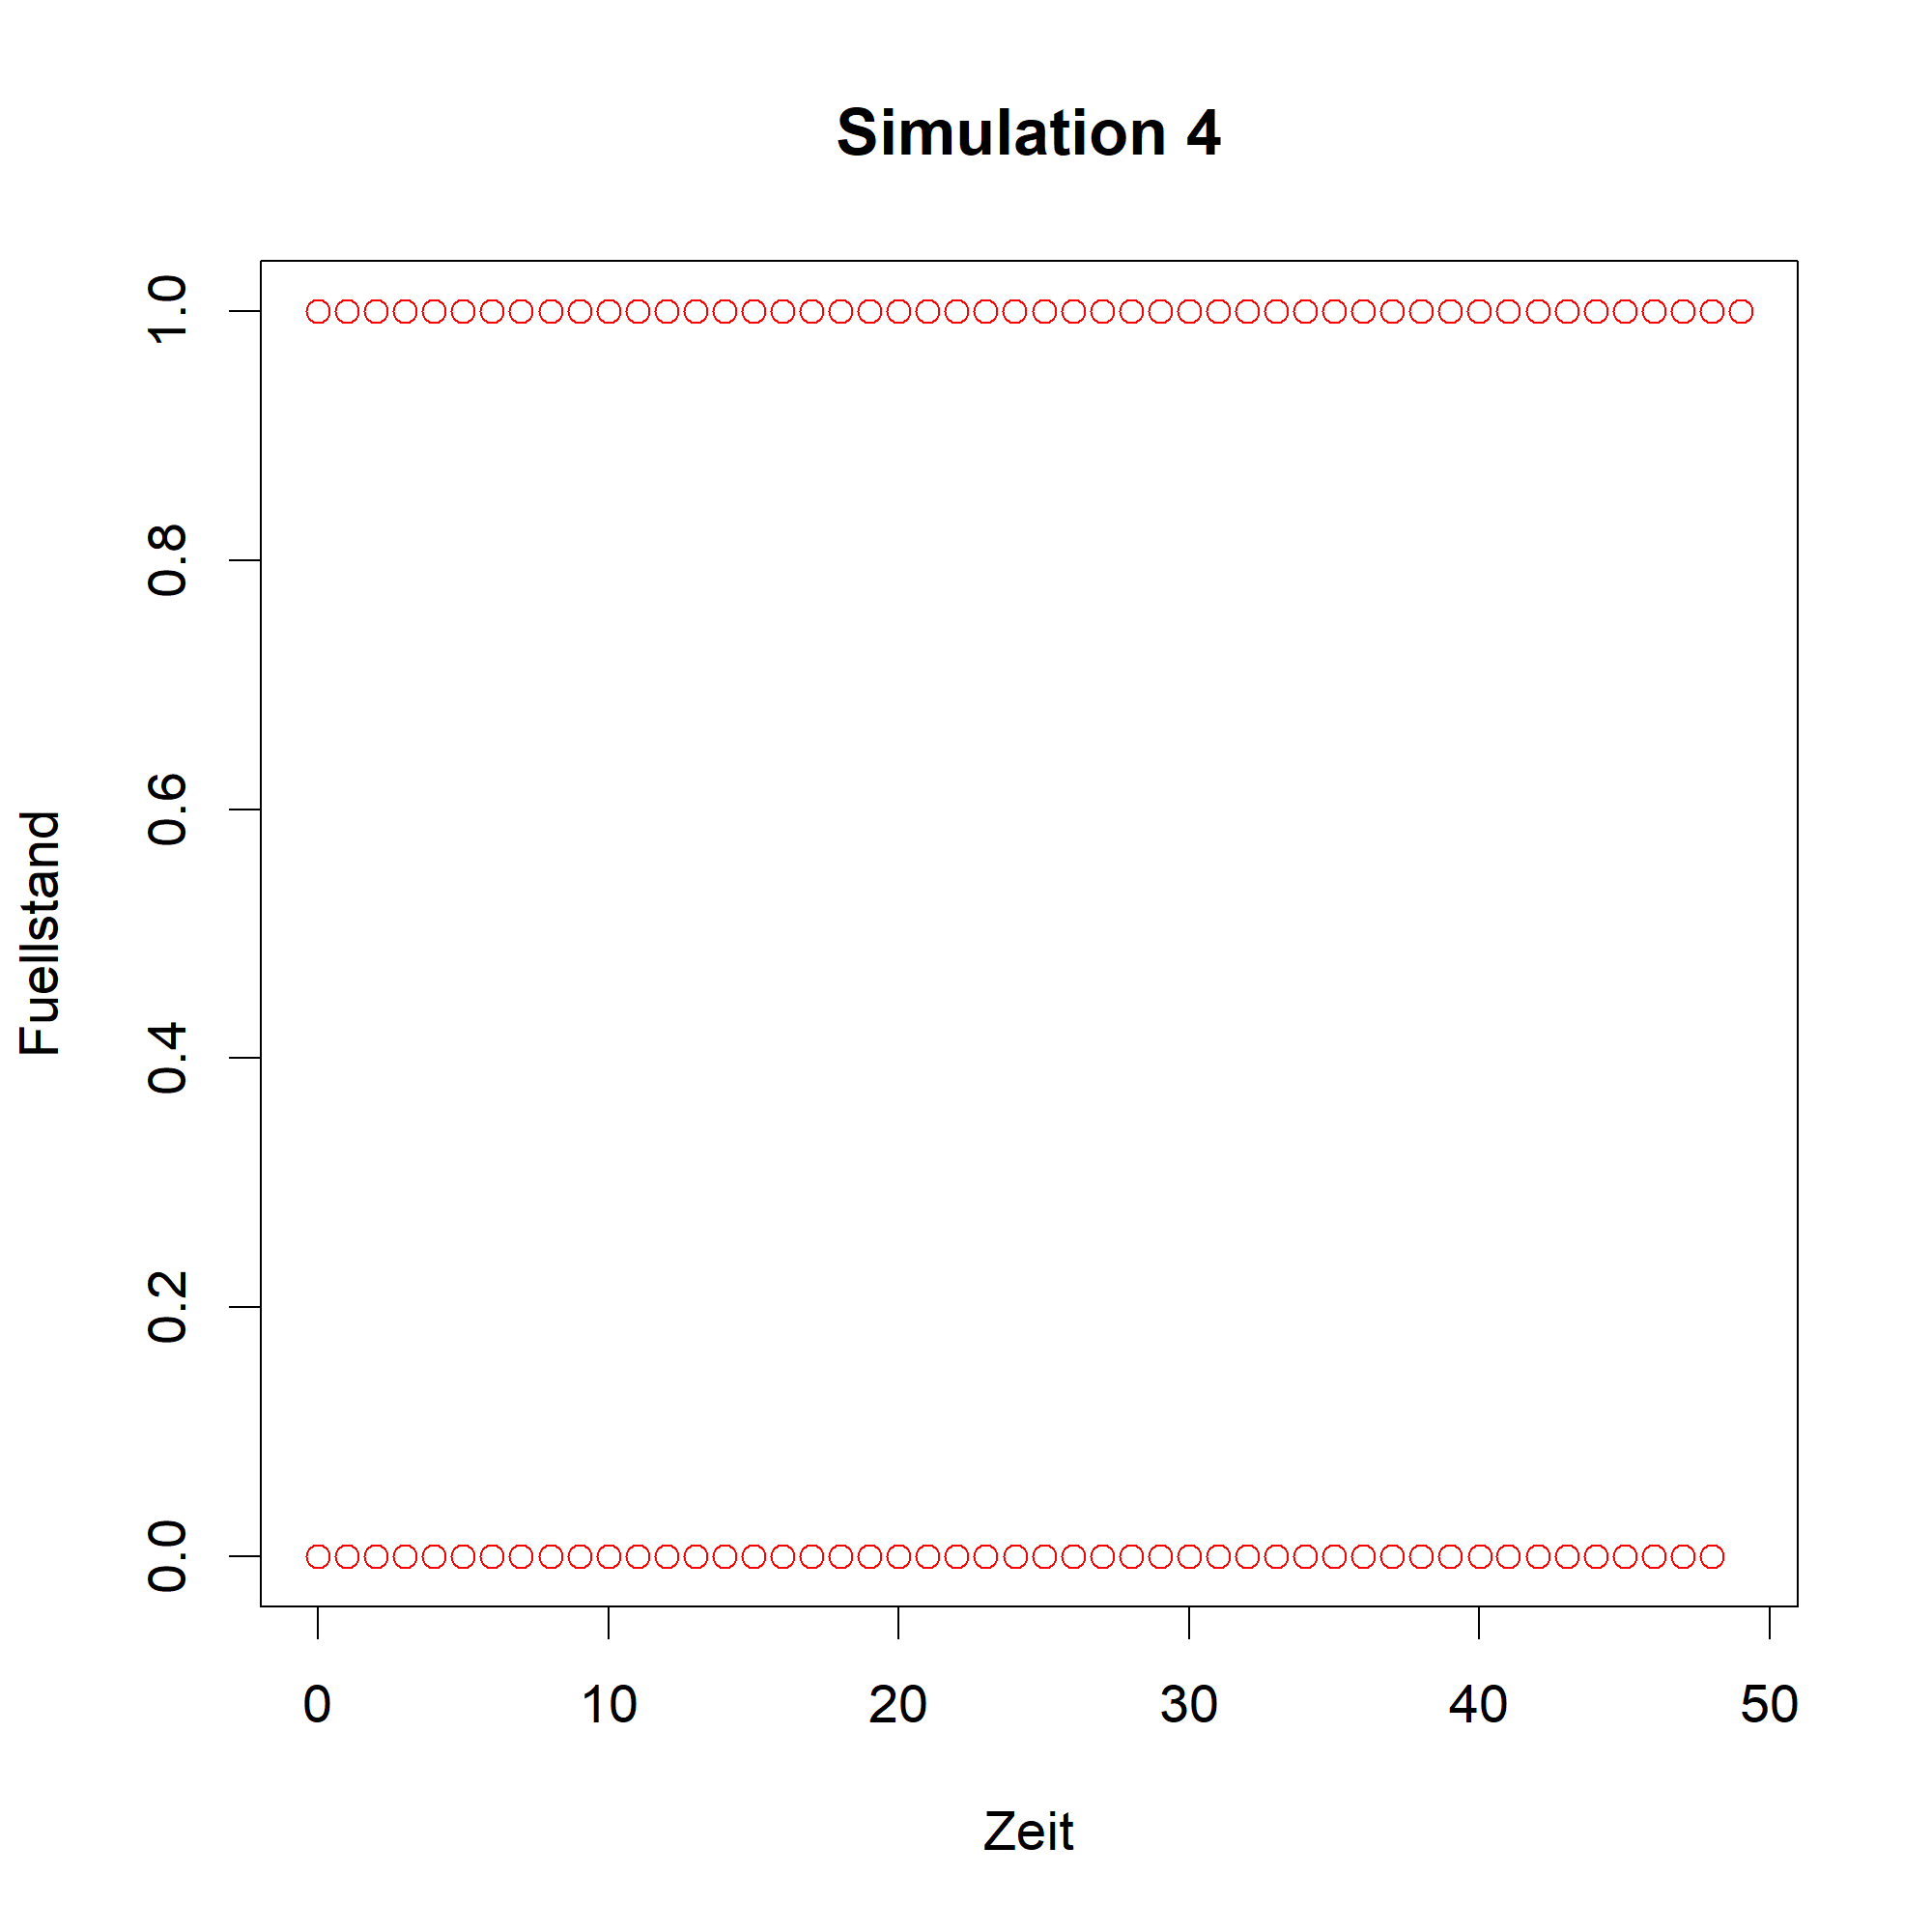
\includegraphics[width=0.7\textwidth]{images/modelSimulationResults/simulation4.png}
 % \caption{Gemeinsames Abarbeiten einer Warteschlange durch zwei Empfaenger (Modell)}
%  \label{img:simulation4}
%\end{figure}

%Simulation 5: \\
%- Max Durchsatz \\
%- eine Nachricht mit max Bytesize schicken \\
%-> Response time sollte kontinuirlich ansteigen \\


\subsubsection{Simulation 5}
Schließlich betrachtet diese Simulation nicht-persistenten Nachrichten. Sender und Empfänger haben die gleiche Ankunftszeiten und kommen einmal pro Sekunde an. Die gesendete Nachrichten haben die Größe 100, 200, 300, 400, 500 und 1000 KByte. Die Ressourcenanforderung für eine Nachricht wurde im Modell angepasst. Dieser ist in \autoref{sec:rmqRd} beschrieben. Verglichen wurde mit der Messung aus \autoref{sec:persistent}. Betrachtet wurde die Latenz der Nachrichten und der Füllstand der Warteschlange. \par
%B
Die Warteschlange bleibt bei dieser Simulation leer. In \autoref{img:simulation6} sind die Ergebnisse bezüglich der Latenz abgebildet. Neben den Vorhersage aus dieser Simulation und den Messpunkte aus der Messung mit persistenten Nachrichten, ist die Vorhersage aus \autoref{sec:rmqSimulation1} eingetragen. In \autoref{tab:sim5} sind die Fehler abgebildet. Dabei wird neben dem Fehler der Vorhersage mit persistenten Nachrichten auch der Fehler zwischen der Messung mit persistenten Nachrichten und der Vorhersage aus \autoref{sec:rmqSimulation1} berechnet. Dabei ist zunächst zu sehen, dass der Fehler zwischen der Messung und der Vorhersage mit persistenten Nachrichten zwischen 10.14\% und 22.12\% liegt. Der Fehler zwischen der Messung mit persistenten Nachrichten und der Vorhersage aus \autoref{sec:rmqSimulation1} liegt zwischen 7.38\% und 15.78\% und ist somit besser. Obwohl der Fehler im zweiten Fall geringer ist, kann dieser nicht genommen werden, da er auf einer falschen Annahme beruht.
\begin{figure}
\center
  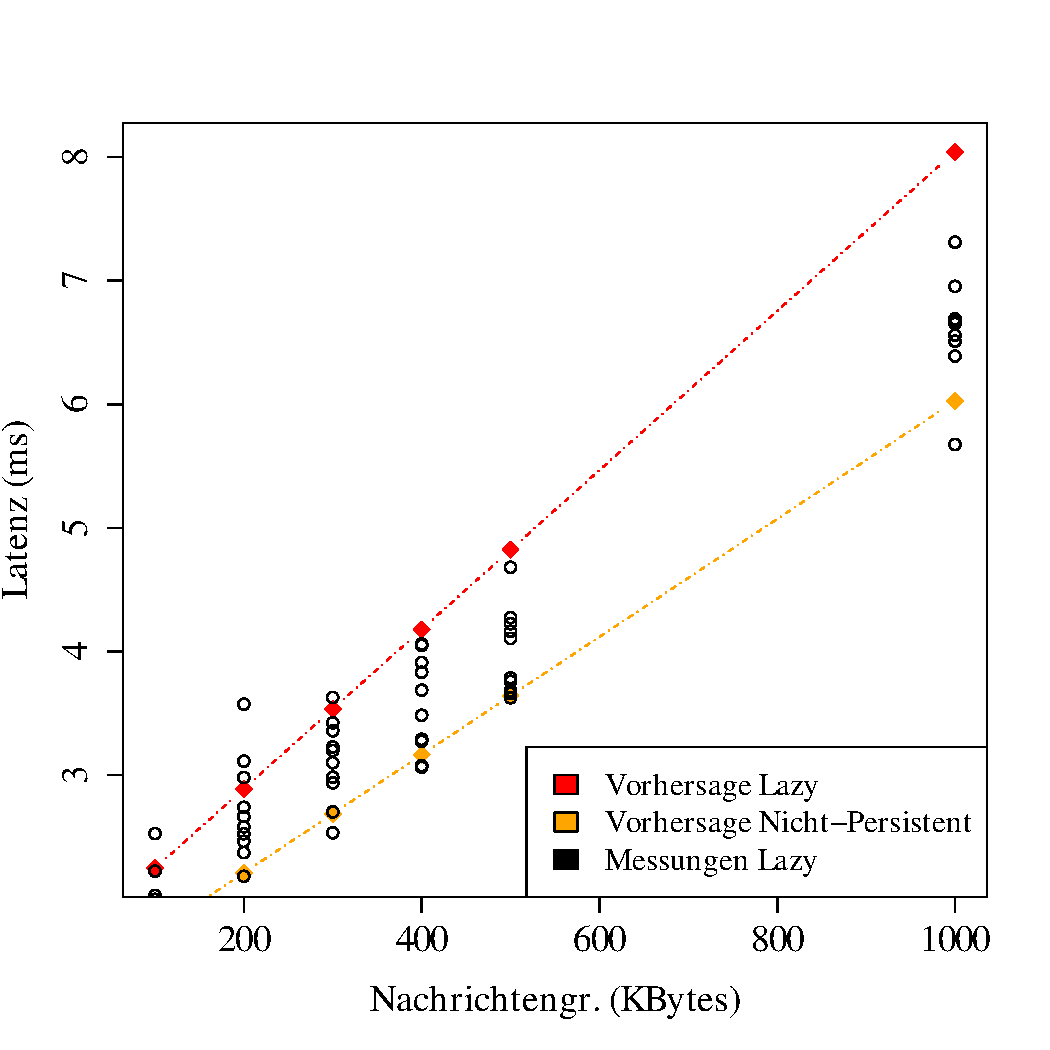
\includegraphics[width=0.7\textwidth]{images/modelSimulationResults/simulation6.pdf}
  \caption{Messung und Vorhersage der Latenz einer persistenten Nachricht mit verschiedenen Größen.}
  \label{img:simulation6}
\end{figure}

\begin{table}
  \begin{tabular}{| l | l | l | l |l | l | l |}
    \hline
    Nachrichtengröße (KB) & 100 & 200 & 300 & 400 & 500 & 1000 \\ \hline
    Messung (\mu s) & 1871,5 & 2624,5 & 3150 & 3586,5 & 3946,5 & 6663,5\\ \hline
    Vorhersage (\mu s) & 2246,59 & 2890,68 & 3534,77 & 4178,85 & 4822,94 & 8043,38\\ \hline
    Fehler (\%) (persistent) & 20,04 & 10,14 & 12,21 & 16,52 & 22,21 & 20,71\\ \hline
    Fehler (\%) (n-persistent) & 7,38 & 15,78 & 14,69 & 11,77 & 7,73 & 9,56\\ \hline
    
    
    \hline
      \end{tabular}
	\caption{\label{tab:sim5} Fehler in \% zwischen Messung und Vorhersage für Simulation 5}
\end{table}


\section{Diskussion}
Die in diesem Kapitel vorgestellt Modellierung einer MOM erfüllt die zu Beginn definierten Anforderungen an eine MOM. Da eine Warteschlange explizit modelliert wurde, können Sender und Empfänger asynchron Nachrichten senden und empfangen. Im Modell ist dies durch unterschiedliche Angabe von Ankunftszeiten möglich. Die zu sendenden Nachrichten können an unterschiedliche Warteschlangen gesendet werden. Dies wurde durch Einsatz von \emph{UsageVariable} und einem \emph{GuardedBranch} im \emph{SEFF} der Exchange Komponente gelöst. Diese Warteschlangen Angabe kann der Benutzer bereits im Nutzungsmodell angeben, zusammen mit der Nachrichtengröße der zu sendenden Nachricht. Wie die Performance-Analyse gezeigt hat, kann sowohl der Füllstand der Warteschlange, als auch die Latenz einer Nachricht, anhand der Modellierung und Kalibrierung, ermittelt werden. Somit konnten die definierten Anforderungen erfüllt werden. Neben den Anforderungen aus diesem Kapitel wurden in \autoref{ch:mom} Einflussfaktoren auf die Performance der MOM identifiziert. Nicht alle Einflussfaktoren, können mit dem aktuellen Ansatz und den aktuell verfügbaren PCM-Modell-Elementen  abgebildet werden. Dazu gehört der Effekt, dass Nachrichten, die lange in der Warteschlange bleiben, eine höhere Latenz haben. Wie die Simulation in \autoref{sec:simulation3} gezeigt hat, kann der Füllstand der Warteschlange zwar richtig angezeigt werden, die erhöhte Latenz dagegen nicht. Ein weiterer Faktor ist die Begrenzung der Warteschlangengröße. Da in dieser Modellierung die Warteschlange als \emph{PassiveRessource} modelliert ist, ist die Angabe einer Größe nicht möglich. Um diese beiden Faktoren abbilden zu können benötigt es eine Erweiterung des PCM und der darauf basierenden Performance-Analyse, mit der eine Warteschlange explizit als Modellelement vorhanden sein muss. Diese Warteschlange kann dann konfiguriert werden mit Topic, Warteschlangengröße und weiteren Konfigurationen. Eine erweiterte Performance-Analyse könnte die Effekte einzelner Nachrichten untersuchen, die eine bestimmte Dauer in der Warteschlange verbracht haben. Dennoch lassen sich mit dieser Modellierung und der ausgewählten Performance-Analyse viele Effekte abbilden, wie die Simulationen in \autoref{sec:performanceanalyse} gezeigt haben. Außerdem wurde gezeigt, dass der Vorhersagefehler unter 33,43\% liegt. Der in der Literatur akzeptierte Vorhersagefehler liegt zwischen 35\% und 40\% \cite{error}. \par
Die vorgestellte Modellierung einer MOM ist jedoch sehr aufwändig. Ein Software-Architekt muss sich viele Gedanken machen, wie viele Warteschlangen, Exchanges und Nachrichtentypen er braucht und muss bei großen Systemen oder vielen Nachrichtentypen viele Verzweigungen in den jeweiligen Exchange-Komponenten modellieren. Im Folgenden Kapitel wird beschrieben, wie mithilfe einer Modeltransformation und dem wiederverwenden der PCM-Event-Elemente, der Komplexität entgegengewirkt werden soll.
%(-- RabitMQ Config:)\\% https://www.rabbitmq.com/configure.html\\
%(-- Kafka Config:)\\ %https://kafka.apache.org/documentation/#brokerconfigs 

